%% makeindex these0.nlo -s nomencl.ist -o these0.nls -t these0.nlg
%!TEX spellcheck = en_US
%!TEX root = thesis.tex

\documentclass[11pt, twoside, openright]{thesis}

% --------------------------------------
% Packages
\usepackage{psl-cover}
\usepackage{lmodern}
\usepackage{appendix}

\usepackage{amssymb}
\usepackage{amsmath}
\usepackage{amsthm}

\usepackage{todonotes}

% --------------------------------------

\definecolor{maincolor}{RGB}{36, 56, 141}
\colorlet{secondarycolor}{violet}

%%%==============================
\title{My PhD Thesis}

\institute{l’École Normale Supérieure de Paris}
\doctoralschool{Sciences Mathématiques de\\ Paris Centre}{386}
\specialty{Informatique}

\author{My Name}
\date{10 Juin 2022}
\jurymember{1}{Name 1}{Université 1}{Rapporteur}
\jurymember{2}{Name 2}{Université 2}{Rapporteur}
\jurymember{3}{Name 3}{Université 3}{Examinatrice}
\jurymember{4}{Name 4}{Université 4}{Directeur de thèse}

% Abstract/Résumé/Mots-clés/Keywords
\frabstract{
%Résumé
}
\enabstract{
%Abstract
\vfill
}
\frkeywords{mots-clés {\Large\color{maincolor}$\star$} mots-clés}
\enkeywords{keywords {\Large\color{maincolor}$\star$} keywords}

%%%==============================
\begin{document}
\frontmatter 
\hypersetup{pageanchor=false}
\maketitle
\hypersetup{pageanchor=true}
\dominitoc

% \begin{dedication}
%   Dedication... 
% \end{dedication}

% =============================================
%                 BEGIN
% =============================================

\cleardoublepage
\chapter*{Résumé}
\addstarredchapter{Résumé}
\thefrabstract{}
\vfill
\thefrkeywords{}
\cleardoublepage
\chapter*{Abstract}
\addstarredchapter{Abstract}
\theenabstract{}
\vfill
\theenkeywords{}

\cleardoublepage
\chapter*{Acknowledgments}
\addstarredchapter{Acknowledgments}

\cleardoublepage
\hypertarget{contents}{}
\tableofcontents

% \printnomenclature % pour faire une page d'index surement
% \mtcfixnomenclature % necessaire pour éviter le decalage des minitoc

%% ====   Corps du texte   === %%
\mainmatter

% !TeX_ROOT=../thesis.tex

\newcommand{\TODO}[1]{\todo[inline, color=orange!30]{\textbf{TODO:} #1}}
\newcommand{\Question}[1]{\todo[inline, color=red!30]{\textbf{Question:} #1}}



% Classical Spaces
\newcommand{\B}{\mathbb{B}}
\newcommand{\Z}{\mathbb{Z}}
\newcommand{\T}{\mathbb{T}}
\newcommand{\R}{\mathbb{R}}

% Distributions
\newcommand{\unif}[1]{\mathcal U \left ( #1 \right )}


% Problems / Ciphertexts
\newcommand{\LWE}{\textsf{LWE}}
\newcommand{\TrivialLWE}{\textsf{TrivialLWE}}
\newcommand{\RLWE}{\textsf{RLWE}}
\newcommand{\GLWE}{\textsf{GLWE}}
\newcommand{\GGSW}{\textsf{GGSW}}

% Classical Mathematical Operations
\newcommand{\rounding}[1]{\left \lfloor #1 \right \rceil}
\newcommand{\drawfrom}{\overset{\$}{\leftarrow}}



% TFHE-specific notations
\newcommand{\lweSigma}{\sigma_{\LWE}}
\newcommand{\glweSigma}{\sigma_{\GLWE}}
\newcommand{\baseDecomp}{B}
\newcommand{\levelDecomp}{\ell}


\newcommand{\lweSecretKey}{\vec s}
\newcommand{\glweSecretKey}{\vec S}

\newcommand{\BSK}{\textsf{BSK}} 
\newcommand{\KSK}{\textsf{KSK}} 
% TODO : trouver une otation pl^us jolie pour BSK


%TFHE homomorphic operations

\newcommand{\sumTFHE}[2]{\texttt{SumTFHE}(#1, #2)}
\newcommand{\sumTFHETernary}[3]{\texttt{SumTFHE}(#1, #2, #3)}
\newcommand{\sumTFHEQuad}[4]{\texttt{SumTFHE}(#1, #2, #3, #4)}
\newcommand{\clearMultTFHE}[2]{\texttt{ClearMultTFHE}(#1, #2)}

\newcommand{\squarewithdot}{\tikz[baseline=-0.5ex]\draw (0,0) rectangle (0.3,0.3) (0.15,0.15) circle (0.05);}

% other operations
\newcommand{\decomp}[3]{\textsf{dec}^{(#1, #2)}(#3)}

% TFHE-related spaces\\
\newcommand{\plaintextTorus}{\mathbb{T}_p}
\newcommand{\plaintextRing}{\mathbb{Z}_p}
\newcommand{\plaintextTorusPoly}{\mathbb{T}_p[X] / (X^N + 1)}
\newcommand{\plaintextRingPoly}{\mathbb{Z}_p[X] / (X^N + 1)}
\newcommand{\lweTorus}{\mathbb{T}_q}
\newcommand{\lweRing}{\mathbb{Z}_q}
\newcommand{\glweTorus}{\mathbb{T}_q[X] / (X^N + 1)}
\newcommand{\glweRing}{\mathbb{Z}_q[X] / (X^N + 1)}



% environments
\theoremstyle{definition}
\newtheorem{definition}{Definition}[section]



\chapter{Introduction: Fully Homomorphic Encryption}



\section{Why ?}





\section{Historical Background}



\TODO{a section on security properties (ind-cpa-d, cca, etc...)}



\section{The bootstrapping : breakthrough construction}




%!TeX_ROOT=../thesis.tex

\chapter{Presentation of the TFHE Scheme}
\label{chap:spec_tfhe}

The previous chapter presented insights on Fully Homomorphic Encryption in general, but this thesis will exclusively cover the TFHE scheme.

Presented in \cite{JC:CGGI20, these_chillotti} as an evolution of the FHEW scheme \cite{EC:DucMic15}, TFHE quickly gained traction to become one of the most promising scheme to attain performances good enough to be  used in real-world scenarios. 

At the core of TFHE lies a powerful \textit{Programmable Bootstrapping} operation (PBS). As we presented in Section \ref{sec:gentry_bootstrapping}, it allows to manage the noise in the ciphertexts during the computation, allowing to achieve Fully Homomorphic Encryption. In TFHE, this bootstrapping operation goes a step further: it enables the evaluation of arbitrary functions directly on the refreshed ciphertexts, with no computational or noise overhead.

In this chapter we provide an in-depth presentation of the TFHE scheme. We introduce the hardness assumptions it relies on, its encryption procedure as well as its homomorphic capabilities. We conclude with insights into its practical performance.

\section{Hardness Assumptions: $\LWE$ and $\GLWE$ Problems}
\label{sec:hardness_assumptions}


\paragraph{Original $\LWE$ problem.}

In 2005, Regev laid the foundations for an important part of modern lattice-based cryptography by defining the Learning With Errors ($\LWE$) problem in \cite{regev_lwe}. The version usually used in FHE literature is presented in Definition \ref{def:LWE}:


\begin{definition}
	(Learning with Errors). Let $q$ and $n$ two integers, respectively called \textit{modulus} and \textit{dimension}.  Let $\chi_s$ and $\chi_e$ be distributions over \textit{small} values of $\lweRing$. We consider a secret vector, sampled as: $\lweSecretKey = (s_0, \dots, s_{n-1}) \drawfrom \chi_s^n$. The $\LWE$ distribution $\mathcal{D}_{q, n, \chi_s, \chi_e}^{\LWE}(\lweSecretKey)$ is defined as:
	
	 \[
	 \mathcal{D}_{q, n, \chi_s, \chi_e}^{\LWE}(\lweSecretKey) = \left \{(\vec a, b) \;\middle|\; \vec a = (a_0, \dots, a_{n-1}) \drawfrom \unif{\lweRing}^n, e \drawfrom \chi_e, b = \innerProduct{\vec a}{\vec s} + e \right \}
	  \]
	 
	 The \textit{decisional} version of the problem is to distinguish this distribution from a uniformly random one, namely:
	
	\[
	\mathcal{D}^{(\textsf{random})} = \left \{(\vec a, r) \;\middle|\; \vec a \drawfrom \unif{\lweRing}^n, r \drawfrom \unif{\lweRing} \right\}
	\]

	The \emph{search} version of the problem is to recover $\lweSecretKey$ from samples of $\mathcal{D}_{q, n, \chi_s, \chi_e}^{\LWE}(\lweSecretKey)$. 
	\label{def:LWE}
\end{definition}


Regev proved that the search and decisional problems are reducible to each other and their average case is as hard as worst-case lattice problems.

The hardness of this problem depends on the parameters $q$, $n$, $\chi_s$ and $\chi_e$, and so does the security of the schemes built upon it. There is not yet in the literature simple guidelines to construct secure instances of the problem. Common practice in the field is to derive an approximate concrete security level $\lambda$ for a given parameter set with a tool named \texttt{lattice-estimator} \cite{lattice-estimator}. Users can input concrete values and distributions for the parameters, and the tool evaluates the security of the underlying $\LWE$ instance by running simulations of attacks of the literature.

In Definition \ref{def:LWE}, we did not specify the shapes of the distributions $\chi_s$ and $\chi_e$ (beyond the fact they yields small values). Several distributions are possible: a discrete Gaussian with a small variance, a uniform distribution restricted on a small interval, or a binomial. Some versions with sparse secrets also exist. The choice of the right distribution depends of the considered use-case, each possibilities offering different trade-offs in matter of security and efficiency \cite{AFRICACRYPT:BGPW16, DBLP:conf/ccs/CurtisP19, EPRINT:BGPT19, EPRINT:SLZS24}.


Most implementations of TFHE select a uniform distribution on $\{0, 1\}$ for the secret, and a Gaussian with a small variance $\lweSigma^2$ for the noise. We will use these distributions in this thesis, and will use the notation $\LWE_{(q, n, \sigma)}$ for these instances.



\paragraph{Extension to the Polynomials.}


Looking for more efficient solutions, $\LWE$ problem has been declined in a \textit{ring variant} named $\RLWE$ in \cite{rlwe}. A generalized version over rings named $\GLWE$, first formalized in \cite{EPRINT:BraGenVai11} and used by TFHE, is presented below. It is very similar to the $\LWE$ one, but deals with polynomial values instead of integers:

\begin{definition}
	(Generalized Learning with Errors) Let $q$, $k$ and $N$ three integers, respectively called \textit{modulus}, \textit{dimension} and \textit{degree}. We consider the polynomial ring $\glweRingFull$, that we denote in short $\glweRing$. Let $\chi_S$ and $\chi_E$ be distributions over the small values of $\glweRing$, (that is to say, polynomials with small coefficients). We consider a secret vector $\glweSecretKey$, sampled as $\glweSecretKey = (S_0, \dots, S_{k-1}) \drawfrom \chi_S^k$. The $\GLWE$ distribution $\mathcal{D}_{q, k, N, \chi_S, \chi_E}^{\GLWE}(\glweSecretKey)$ is defined as:
	
	\[
	\mathcal{D}_{q, k, N, \chi_S, \chi_E}^{\GLWE}(\glweSecretKey) = \left \{ (\vec A, B) \;\middle|\; \vec A = (A_0, \dots, A_{k-1}) \drawfrom \unif{\glweRing}^k, E \drawfrom \chi_E, B = \innerProduct{\vec A}{\vec S} + E \right \}
	\]
	
	The \textit{decisional} version of the problem is to distinguish this distribution from a uniformly random one, namely:
	
	\[
	\mathcal{D}^{(\textsf{random})} = \left \{(\vec A, R) \;\middle|\; \vec A \drawfrom \unif{\glweRing}^k, R \drawfrom \unif{\glweRing} \right\}
	\]
	
	The \emph{search} version of the problem is to recover $\lweSecretKey$ from samples of $\mathcal{D}_{q, k , N, \chi_S, \chi_E}^{\GLWE}(\glweSecretKey)$. 
	\label{def:GLWE}
\end{definition}

Note that if we fix $k = 1$, we fall back on the classical $\RLWE$ problem, notably used in BGV \cite{bgv}. Also, taking $N=1$ produces a $\LWE$ instance with $n = k$. 

Concretely, using polynomial rings allows to encode more information in a single sample, yielding more compact ciphertexts and public keys. The schemes can also benefit from high-speed polynomial arithmetic techniques such as Fast Fourier Transforms (FFT). 

General consensus is that hardness of an instance $\GLWE_{(q, k, N, \sigma)}$ is similar to the hardness of $\LWE_{(q, k \cdot N, \sigma)}$, which makes possible to use the \texttt{lattice-estimator} as well.


\section{Torus Equivalence and Discretization}
\label{sec:torus_equivalence}


The T in TFHE stands for \textit{Torus}, because in the seminal paper of TFHE \cite{JC:CGGI20}, authors worked with torus-based variants of $\LWE$ and $\GLWE$.


The torus $\T = \R / \Z$ corresponds to the reals modulo 1. Algebraically, this space does not have a ring structure, but actually is a \textit{$\Z$-module} one, which means that:

\begin{itemize}
	\item The sum of two torus elements is well-defined, and yields another torus element.
	\item The multiplication between an element of $\T$ and an element of $\Z$ is also well-defined, and produces an element of $\T$.
	\item On the other hand, multiplying two elements of $\mathbb T$ does not make sense. To be convinced of it, we can remark that, for any non-zero torus element $x$, $0 \times x = 0$ while $1 \times x = x$. But since 0 and 1 are equivalent over the torus, these results should not be different. 
\end{itemize}



Recall the $\LWE$ assumption (Definition \ref{def:LWE}). If we rescale the elements of $\lweRing$ by dividing them by $q$, we get torus elements. We can then redefine seamlessly the $\LWE$ problem over the torus. Extensive details about this transformation can be found in \cite{these_chillotti}.


This brings two advantages:

\begin{itemize}
	\item $\LWE$ over the torus is \textit{scale-invariant}, which makes the analysis of the security and of the noise much simpler.
	\item The $\Z$-module structure propagates in the ring versions, as well as in matrices spaces. Thus, it allows for very powerful generalizations of homomorphic schemes on a wide variety of spaces, like in \cite{chimera, chimera2}.
\end{itemize} 


When implementing the scheme in practice, torus elements are represented by integers in machine. The torus is thus seen as \textit{discretized}, which we denote by 

\[ \T_q = \left \{   \frac a q \;\middle|\; a \in \Z_q  \right \} \] 

with $q = 2^\Omega$ ($\Omega$ denotes the number of bits of precision of the type, so 32 or 64 bits in most implementations). The properties of the torus structure are preserved.


This thesis is mainly about practical instantiations of the scheme. So, for the sake of clarity we will adopt a notation closer to the reality of the objects manipulated in machine. So the torus elements will be seen as elements of $\lweRing$ (but keeping the algebraic rules imposed by the structure of $\T$), and the same will be applied for ring extensions. 



\section{Encryption and Decryption in TFHE}
\label{sec:encryption}

\paragraph{Spaces.}

To understand the encryption procedure of TFHE, we must first introduce its plaintext space and its ciphertext space, and how the former can be embedded into the latter.

The plaintext space of TFHE is the \textit{discretized torus} $\plaintextTorus$. As explained in Section \ref{sec:torus_equivalence}, we trivially identify it to the ring $\plaintextRing$ with $p$ an integer. Conversely, the ciphertext space is the discretized torus $\lweTorus$ introduced in the previous section identified to a ring $\lweRing$, with $q = 2^\Omega$. In practice, $p \ll q$.


We need a way to encode plaintext values into the ciphertext space. To do so, let us consider a mapping $\rho: \plaintextRing \rightarrow \lweRing$, defined as \[
\rho: m  \mapsto \rounding{\frac{m \cdot q} {p}}.
\]


The image of this mapping only reaches $p$ elements in $\lweRing$, forming the set $\left \{ \rounding{\frac {k q}{p}} \mid k \in \plaintextRing \right \}$. These elements are distributed around $\lweRing$ and form what we refer to as \emph{sectors of $\lweRing$}, defined as: \[
\left\{ \left( \frac{(2k - 1)q}{2p}, \frac{(2k + 1)q}{2p} \right) ~\middle|~ k \in \mathbb{Z} \right\}
\]. A representation of such a mapping is shown on Figure \ref{fig:example_encoding}.

To encode a given plaintext element $m$ into the ciphertext space, we use the corresponding center of sector $\rounding{\frac{mq}{p}}$. However, decoding is more permissive: every elements of a sector are decoded by the corresponding plaintext element. This will be useful to remove the noise in ciphertexts.

\begin{figure}[htbp]
	\centering
	\wrappedTorus{64}{8}{true}
	\caption{An example of embedding of $\Z_8$ into $\Z_{64}$}
	\label{fig:example_encoding}
\end{figure}

We can now move to the actual encryption and decryption algorithms. TFHE features two main types of encryption: $\LWE$ encryption and $\GLWE$ encryption. Both share similar structural patterns but operate within different mathematical spaces.

\paragraph{LWE Encryption.}
$\LWE$ encryption deals with scalar values. The plaintext space is $\plaintextRing$ and the secret key is sampled uniformly at random from $\B^n$. We denote by $q$ the ciphertext modulus. We also need 
$\chi_{\lweSigma}$, a centered Gaussian distribution of standard deviation $\lweSigma$ in $\lweRing$. The encryption algorithm produces a ciphertext $\vec c$ of the form:

\begin{definition}($\LWE$ ciphertext)
	A $\LWE$ ciphertext encrypting a message $m \in \plaintextRing$ under a secret key $\lweSecretKey=(s_0, \dots, s_{n-1}) \in \B^n$ has the form:
	
	\begin{equation}
		\vec c = \LWE_{\lweSecretKey}(m) = \left (a_0, \dots, a_{n-1}, b = \sum_{i=0}^{n-1} a_i \cdot s_i + \tilde m + e \right ) \in \lweRing^{n+1}
	\end{equation}
	where:
	\begin{itemize}
		\item the elements $\vec a = (a_0, \dots, a_{n-1})$ are sampled uniformly at random in $\lweRing$.

		\item $\tilde m$ is the message encoded in the ciphertext space: $\tilde m = \rho(m) \in \lweRing$.
		\item $e$ is a small random Gaussian noise sampled from $\chi_{\lweSigma}$.
	\end{itemize}
\end{definition}


Decryption is performed in two steps: first, we compute the \emph{phase} of the ciphertext as $\phi(\vec c) = b - \langle \vec a, \vec s\rangle$. The phase corresponds to the noisy message $\tilde{m} + e$. To recover the actual message, we simply decode the phase by looking up the plaintext element corresponding to the sector. This can be interpreted as a rounding: $m = \rounding{\frac p q \phi(c)}$. 

As long as $|e| < \frac{q}{2p}$, this rounding produces the right sector center, and thus we recover the correct plaintext value. Otherwise the phase lies in a different sector and we recover a wrong value. It is thus very important to keep the noise level low enough to ensure correct decryption.


Security-wise, this encryption relies on the hardness of the assumption $\LWE_{(q, n, \lweSigma)}$. The dimensioning of these parameters should be handled properly to ensure security, correctness and efficiency. Chapter \ref{chap:parameters} of this thesis will be dedicated to this question.



\paragraph{GLWE Encryption.} This encryption mode mirrors the structure of $\LWE$ encryption but operates within polynomial rings.
This time, the plaintext space is $\plaintextTorusPoly$, identified with the ring $\plaintextRingPoly$.

The secret key $\glweSecretKey$ is represented as a vector $(S_0, \dots, S_{k-1})$, sampled uniformly at random from $\B_{N, q}[X]^k$. 
%
The message is encoded in a polynomial $\tilde M \in \glweRing$, with the same encoding process than $\LWE$ (but applied coefficient-wise). The noise is also a polynomial from the same ring, whose coefficients are drawn from the distribution $\chi_{\glweSigma}$.
%

The encryption procedure outputs a ciphertext $\vec C$ of form:


\begin{definition}($\GLWE$ ciphertext)
	A $\GLWE$ ciphertext encrypting a message $M \in \plaintextRingPoly$ under a secret key $\glweSecretKey = (S_0, \dots, S_{k-1}) \in \B_{N, q}[X]^k$ has the form:
	
	\begin{equation*}
		\vec C = \GLWE_{\glweSecretKey}(M) = \left ( A_0, \dots, A_{k-1}, B = \sum_{i=0}^{k-1} A_i \cdot S_i + \tilde M + E \right ) \in \glweRing
	\end{equation*}
	where:
	\begin{itemize}
		\item the elements $\vec A = (A_0, \dots, A_{k-1})$ are sampled uniformly at random in $\glweRing$.
		\item $\tilde M$ is the message encoded in the ciphertext space: $\tilde M = \rho(M)$.
		\item $E$ is a polynomial with small Gaussian coefficients, that are sampled from $\chi_{\glweSigma}$.
	\end{itemize}
\end{definition}



Decryption follows the same steps as the $\LWE$ case: the phase is computed as $\phi(\vec C) = B - \langle \vec A, \vec S \rangle$ and rounded to the closest plaintext value.


The security of this encryption relies on the hardness of the assumption $\GLWE_{(q, k, N, \glweSigma)}$. Because the plaintext is a polynomial of degree $N$, it is possible to trivially batch up to $N$ plaintexts from $\plaintextRing$ by encoding them in the coefficients. With this method, they can be processed in parallel by the linear homomorphism presented below (but not by the bootstrapping!).
\medskip
To give an idea of the size of the objects at play here, $n$ is usually chosen between 500 and 1000, $q$ is usually $2^{64}$ and $N$ is a power of two between $2^8$ and $2^{12}$. Chapter \ref{chap:parameters} is dedicated to the problem of parametrization of the scheme, and gives further explanations on the role and the range of each parameter.

A third encryption flavour, named $\GGSW$ also exists. We introduce it in Section \ref{sec:external_products} where it is necessary.


\section{Linear Homomorphisms}

On a torus, two operations are well-defined: the sum of two torus elements and the external product between a torus element and a \textit{scalar}.

It is not hard to see that both TFHE encryption modes are linearly homomorphic. We define the two operations \texttt{sumTFHE} and \texttt{clearMultTFHE} that we present in the following. We present only the $\LWE$ version, but they can be trivially transposed to $\GLWE$ as well.


\paragraph{$\sumTFHE{\vec c}{\vec c'}$:} Let $\vec c = (a_0, \dots, a_{n-1}, b)$ and $\vec c' = (a_0', \dots, a_{n-1}', b')$ be two $\LWE$ ciphertexts encrypting the messages $m$ and $m'$ from $\plaintextRing$, with respective noise variance $\sigma$ and $\sigma'$. Summing coefficient-wise both ciphertexts yields a new ciphertext $\vec c'' = (a_0 + a_0', \dots, a_{n-1} + a'_{n-1}, b + b')$ encrypting $m + m'$ with a larger noise $e + e'$.


\paragraph{$\clearMultTFHE{c}{\lambda}$:} Let $\vec c = (a_0, \dots, a_{n-1}, b)$ a $\LWE$ ciphertext encrypting a message $m \in \plaintextRing$ and $\lambda \in \plaintextRing$ a constant. Multiplying each coefficient by the constant yields a new ciphertext $\vec c' = (\lambda \cdot a_0, \dots, \lambda \cdot a_{n-1}, \lambda \cdot b)$ encrypting the message $\lambda \cdot m$ with a larger noise $\lambda \cdot e$.


\medskip
These notations will be used throughout this manuscript. However, sometimes when it is clear from the context that we are referring to homomorphic operations, we may use the classical $+$ and $\cdot$ symbols to lighten the formulas.





\section{Key Switching}
\label{sec:keyswitch}

We now introduce a more advanced operation: the $\KeySwitch$. Let $\vec c = \LWE_{\lweSecretKey}(m) = (a_0, \dots, a_{n-1}, b)$ be a $\LWE$ ciphertext encrypting a message $m$ under the secret key $\lweSecretKey$. $\KeySwitch$ allows the server to homomorphically transform $c$ into a new ciphertext $c'$ encrypting the same message $m$ under another secret key $\lweSecretKey'$. This operation is very useful in practical settings: for example it allows to switch between different ciphertext types and shapes to speed up some computations, particularly in the bootstrapping algorithm. It is also central in some multi-client use-cases.

We start by explaining the $\LWE$-to-$\LWE$ version of keyswitching and then generalize to the ring case.


\paragraph{Some intuition on keyswitching.}
The rationale behind the keyswitching algorithm is to homomorphically evaluate the linear part of the decryption function (namely $b - \langle \vec a, \lweSecretKey \rangle$), given an encryption of $\lweSecretKey$ under the key $\vec s'$. This ``encrypted secret key'' is called the \textit{keyswitching key} and is denoted by $\KSK$. Even if it looks a lot like a bootstrapping operation, keyswitching is actually quite different. Notably, it \textit{increases} the noise in the ciphertext (see \cite{JC:CGGI20, these_tap} for concrete noise analysis).


More formally, let $\KSK$ be the vector of encryption of every bit of the key $\lweSecretKey$ under the key $\lweSecretKey'$:

\[
	\KSK = \left \{ \LWE_{\lweSecretKey'}(s_i ) \right \}_{0 \le i < n}
\]

Notice how, if we treat the coefficients $a_i$ (the mask of $\vec c$) as scalar constants, we can homomorphically evaluate the product $- \langle \vec a ,\lweSecretKey \rangle$ with the basic linear operations of TFHE. Moreover, adding the constant $b$ is easy if we remark that the trivial ciphertext $\TrivialLWE(b) = (0, \dots, 0, b)$ is a valid instance of $\LWE_{\lweSecretKey'}(b)$. So the operation $b - \langle \vec a, \lweSecretKey \rangle$ is equivalent in the encrypted world to:


\begin{align*}
	b - \langle \vec a, \vec s \rangle &\sim \TrivialLWE(b) - \innerProduct{ \vec a}{\KSK}\\
	& = \LWE_{\lweSecretKey'}(b - \langle \vec a, \lweSecretKey \rangle)\\
		 &= \LWE_{\lweSecretKey'}(m + e)
\end{align*}


and we effectively get a new encryption of $m$ under $\lweSecretKey'$ (at the cost of some extra noise).


However, there is a problem with this approach: recall that the $a_i$'s are uniformly distributed in the ring $\lweRing$. So they have in average a very large magnitude (about $\frac q 4$). Also recall that the scalar multiplication of TFHE increases the noise by the same factor as the multiplicative constant. So if one uses this first version of keyswitching, the noise would completely skyrocket and the result would be unusable.

Thankfully, there is a well-known way to improve the noise growth in the scalar multiplication: it is called \textit{gadget decomposition}. We introduce it below:

\paragraph{Gadget Decomposition.}

To begin with, we introduce an \textit{exact} version of the gadget decomposition for clarity. The variant used in TFHE is an \textit{approximate} one, which is conceptually only slightly more complex.


Recall that we want to compute the scalar product $a_i \cdot \LWE_{\lweSecretKey}(m)$, with $a_i$ a potentially large value in $\lweRing$, without noise explosion.

The core idea is to work with a \textit{decomposition} of the constant $a_i$ in some basis. Let $(\baseDecomp, \levelDecomp)$ be two integers such that $\baseDecomp^\levelDecomp = q$. We denote the decomposition of $a_i$ in this basis by:

\[
	\decomp{\levelDecomp}{\baseDecomp}{a_i} = (a_{i,0}, \dots, a_{i, \levelDecomp-1}) \text{ such that: } a_i = \sum_{j=0}^{\levelDecomp-1} a_{ij} \cdot \baseDecomp^j
\]

In parallel, instead of working with a single ciphertext $\LWE_{\lweSecretKey}(m)$, we use a collection of $\levelDecomp$ ciphertexts, each encrypting a scaled version of $m$. These ciphertexts are fresh encryption, so they all have the same fresh noise level $\lweSigma$.: 

\[
	\left \lbrace \LWE_{\lweSecretKey}(m \cdot \baseDecomp^j) \right \rbrace_{0 \le j < \levelDecomp}
\]

Now, observe that instead of directly performing the product $a_i \cdot \LWE_{\lweSecretKey}(m)$, we can instead performs the sum 

\[
	\sum_{j=0}^{\levelDecomp - 1} a_{i,j} \cdot \LWE_{\lweSecretKey}(m \cdot \baseDecomp^j) \text{ with: } \decomp{\baseDecomp}{\levelDecomp}{a_i} = (a_{i, 0}, \dots, a_{i, \ell-1})
\]

which yields the correct result. Computing the product this way makes the noise grow only by a factor $\baseDecomp \cdot \levelDecomp$ instead of $a_i$ (at the cost of storing $\levelDecomp$ ciphertexts instead of one).



Note that what we just presented here was a very simple case. A rigorous formalism of gadget decomposition is developed in \cite{EC:GenMicPol19}, and some more analysis can be found in \cite{AC:Joye21}.


One of the innovations of TFHE is the realization that approximating the decomposition yields a significant performance improvement, at the cost of only a slight degradation of the noise. So instead of taking exactly $\baseDecomp^\levelDecomp = q$, we pick smaller values in TFHE such that $\baseDecomp^\levelDecomp < q$.


\paragraph{Back to a better keyswitching.}

Coming back to the keyswitching algorithm, we pick decomposition parameters $(\baseDecomp$, $\levelDecomp)$ and add a dimension to the keyswitching key to store each scaled version. So $\KSK$ becomes:

\[
	\KSK = \left \lbrace \left ( \LWE_{\lweSecretKey'} (s_i \cdot \baseDecomp^0), \dots  \LWE_{\lweSecretKey'} (s_i \cdot \baseDecomp^{\levelDecomp-1}) \right ) \right \rbrace_{0 \le i < n}
\]


and we replace the simple scalar multiplications in the keyswitching algorithm by inner products between the decompositions of each $a_i$ and each member of the keyswitching key. This gives us the full $\LWE$-to-$\LWE$ algorithm, that we detail in Algorithm \ref{alg:keyswitching}



\begin{algorithm}
	\caption{\texttt{$\LWE$-to-$\LWE$ KeySwitching}}
	\label{alg:keyswitching}
	\KwContext{
		$\left\{
			\begin{array}{l}
				\lweSecretKey \text{: the input $\LWE$ secret key}\\
				\lweSecretKey' \text{: the output $\LWE$ secret key}\\
				\levelDecomp \text{: the level of the decomposition}\\
		         \baseDecomp \text{: the base of the decomposition}
		  	\end{array}
		  \right.$
	}
	
    \KwIn{
		$\left\{
		\begin{array}{l}
			c = (a_0, \dots, a_{n-1}, b) \text{: a ciphertext $\LWE_{\lweSecretKey}(m)$} \\
			\KSK = \left\{ \left( \LWE_{\lweSecretKey'} (s_i \cdot \baseDecomp^0), \dots, \LWE_{\lweSecretKey'} (s_i \cdot \baseDecomp^{\levelDecomp-1}) \right) \right\}_{0 \le i < n} \text{: the keyswitching key}
		\end{array}
			\right.$
	}
	
	\KwResult{
		$c_{\textsf{out}}$ \text{: a ciphertext $\LWE_{\lweSecretKey'}(m)$}
	}
	
	
	 % Add vertical space and horizontal line
	 \vspace{0.5em} % adjust the space as needed
	 \hrule
	 \vspace{0.5em} % adjust the space as needed
	
	$c_{\textsf{out}} \gets (0, \dots, 0, b)$
	
	\For{$i \in \lbrace 0, \dots, n-1 \rbrace$}{
	
		$c_{\textsf{out}} \gets c_{\textsf{out}} - \left \langle \decomp{\levelDecomp}{\baseDecomp}{a_i}, \KSK_i \right \rangle$
	}
	
	\Return{$c_{\textsf{out}}$}	
\end{algorithm}




\paragraph{Generalization to $\GLWE$.}


We introduced keyswitching in its $\LWE$-to-$\LWE$ form, but everything generalizes nicely to construct a $\LWE$-to-$\GLWE$ flavour. Here, $\KSK$ is a collection of $\GLWE$ ciphertexts, and the decomposition is applied coefficient-wise on the polynomials. The resulting $\GLWE$ ciphertext encrypts a polynomial whose degree-zero coefficient encodes the original message.


It is then possible to pack several $\LWE$ ciphertexts into a single $\GLWE$ one, by multiplying the results by different monomials to move the encoded coefficient in a higher degree. They can then be summed. This is known in the literature as the $\PackingKeySwitch$. As this will be useful particularly in Chapter \ref{chap:hyppogriph}, we detail it in Algorithm \ref{alg:packing_keyswitching}.

\begin{algorithm}
	\caption{$\PackingKeySwitch$}
	\label{alg:packing_keyswitching}
	\KwContext{
		$\left\{
		\begin{aligned}
			&\lweSecretKey \text{: the input $\LWE$ secret key}\\
			&\glweSecretKey' \text{: the output $\GLWE$ secret key}\\
			&\levelDecomp \text{: the level of the decomposition}\\
			&\baseDecomp \text{: the base of the decomposition}
		\end{aligned}
		\right.$
	}
	
	\KwIn{
		$\left\{
		\begin{aligned}
			&\left \lbrace \vec c_i = \LWE_{\lweSecretKey}(m_i) \right \rbrace_{0 \le i < \alpha} \text{: a list of $ \alpha~\LWE$ ciphertexts to be packed, with $\alpha \le N$} \\
			&\KSK = \left\{ \left( \GLWE_{\glweSecretKey'} (s_i \cdot \baseDecomp^0), \dots, \GLWE_{\glweSecretKey'} (s_i \cdot \baseDecomp^{\levelDecomp-1}) \right) \right\}_{0 \le i < n} \text{: the keyswitching key}
		\end{aligned}
		\right.$
	}
	
	\KwResult{
		$\vec C_{\textsf{out}}$ \text{: a $\GLWE$ ciphertext encrypting the list of messages $\lbrace m_i \rbrace_{0 \le i < \alpha}$}
	}
	
	
	% Add vertical space and horizontal line
	\vspace{0.5em} % adjust the space as needed
	\hrule
	\vspace{0.5em} % adjust the space as needed
	
	$\vec C_{\textsf{out}} \gets 0$\\
	\For{$k \in \lbrace 0, \dots, \alpha-1 \rbrace$}{
		$\vec C_{k}' \gets \KeySwitch(\vec c_k, \KSK)$\\
		$\vec C_{\textsf{out}} \gets \vec C_{\textsf{out}} + X^k \cdot \vec C_{k}'$
	}
	
	\Return{$\vec C_{\textsf{out}}$}	
\end{algorithm}


More possibilities exist in the literature: notably generalizing Algorithm \ref{alg:keyswitching} to define a $\GLWE$-to-$\GLWE$ flavour. It is also possible to evaluate functions while keyswitching by applying it on the decomposed scalars (making it a \textit{public} functional keyswitch) or on the encryption of the bits of the original secret key (making it a \textit{private} one). An in-depth tour of keyswitches can be found in \cite{these_tap}.


\section{External Products}
\label{sec:external_products}

In the previous section, we showed how the use of gadget decomposition allowed for practical multiplications by constant. Actually, we can push it further: by using decompositions of ciphertexts themselves, it becomes possible to multiply two ciphertexts together! By reference to the original GSW scheme \cite{C:GenSahWat13}, these decomposed ciphertexts are called $\GGSW$ ciphertexts (for \textit{Generalized GSW}).


We start by formalizing a bit more the notion of gadget decomposition: while several decomposition algorithms exist on the literature, we focus in this thesis on the most classical one (called \textit{canonical} in the seminal paper of TFHE). We recall its definition:

	
\begin{definition}(Gadget Matrix)\\
	Let $\Z_{q, N}[X]^{k+1}$ be the domain of $\GLWE$. Let the two positive integers $\levelDecomp$ and $\baseDecomp$ be the base of the gadget. The gadget is the list of $(k+1) \levelDecomp$ rows of the matrix $\mat H \in \Z_{N, q}[X]^{(k+1)\levelDecomp \times k+1}$ defined by:
	
	\[
	\mat H = 
	\left(
	\begin{array}{c|c|c}
		q / \baseDecomp & \dots & 0 \\
		\vdots & \ddots & \vdots  \\
		q / \baseDecomp^{\levelDecomp} & \dots & 0 \\
		\hline
		\vdots & \ddots & \vdots \\
		\hline
		0 & \dots & q / \baseDecomp \\
		\vdots & \ddots & \vdots  \\
		0 & \dots & q / \baseDecomp^{\levelDecomp}\\
	\end{array}
	\right) \in \Z_{N, q}[X]^{(k+1)\levelDecomp \times k+1}
	\]
\end{definition}
	


Using this matrix, it is possible to define a new type of ciphertexts, called $\GGSW$ ciphertexts. We give their classical definition below:


\begin{definition}($\GGSW$ ciphertexts)
	\label{def:ggsw}
	Let $(\baseDecomp, \levelDecomp)$ an approximate decomposition base. A $\GGSW$ ciphertext $\mat C$ encrypting a message $M \in \plaintextRingPoly$ under a GLWE secret key $\glweSecretKey =  (S_0, \dots, S_{k-1}) \in \B_{N, q}[X]^k$ has the form:
	\begin{equation*}
		\mat C = \mat Z + M \cdot \mat H
	\end{equation*}
	where each row of $\mat Z$ is a valid $\GLWE$ ciphertext of 0 for the key $\glweSecretKey$. 
	
\end{definition}


In more recent works (for example \cite{AC:CLOT21} and its follow-ups), an alternative (but equivalent) definition is used. We reproduce it here as well:

\begin{definition}($\GGSW$ ciphertext, second definition)
	\label{def:ggsw2}
	Let $(\baseDecomp, \levelDecomp)$ an approximate decomposition base. A $\GGSW$ ciphertext encrypting a message $M \in \plaintextRingPoly$ under a GLWE secret key $\glweSecretKey =  (S_0, \dots, S_{k-1}) \in \B_{N, q}[X]^k$ has the form:
	
	\begin{equation*}
		\GGSW_{\glweSecretKey}(M) = \left \lbrace \left ( \GLWE_{\glweSecretKey}\left (-S_\alpha \cdot M \cdot \frac{q}{\baseDecomp^j} \right) \right )_{0 \le j < \levelDecomp} \right \rbrace_{0\le \alpha \le k}
	\end{equation*}
	
	with $S_{k+1}$ fixed by convention to -1.
\end{definition}


These ciphertexts allow the definition of an \textit{external product}. It is possible to multiply a $\GGSW$ ciphertext (encrypting a message $M_1$) with a $\GLWE$ one (encrypting a message $M_2$) to obtain another $\GLWE$ ciphertext that encrypts the product $M_1 \cdot M_2$. We denote this operation by:

\begin{equation*}
		\boxdot: \GGSW \times \GLWE \rightarrow \GLWE
\end{equation*}


Algorithm \ref{alg:external_product} details this procedure. As for $\KeySwitch$, External Product increases the noise in the ciphertexts. Again, exact noise formulas can be found in \cite{JC:CGGI20, these_tap}. The line of work of \cite{chimera, AC:BCGGJ24} gives a nice mathematical overview of how these decompositions techniques can be interpreted as lifts from the $\Z$-module structure to the underlying ring. 

\begin{algorithm}
	\caption{\texttt{External Product}}
	\label{alg:external_product}
	\KwContext{
		$\left\{
		\begin{array}{l}
			\glweSecretKey \text{: the input $\GLWE$ secret key}\\
			\levelDecomp \text{: the level of the decomposition}\\
			\baseDecomp \text{: the base of the decomposition}
		\end{array}
		\right.$
	}
	
	\KwIn{
		$\left\{
		\begin{array}{l}
			C = (A_0, \dots, A_{k-1}, B) \text{: a ciphertext }\GLWE_{\glweSecretKey}(M_1) \\
			CT = \left \lbrace \left ( \GLWE_{\glweSecretKey}\left (-S_\alpha \cdot M \cdot \frac{q}{B^j} \right) \right )_{0 \le j < \levelDecomp} \right \rbrace_{0\le \alpha \le k+1} \text{: a ciphertext } \GGSW_{\glweSecretKey}(M) 
		\end{array}
		\right.$
	}
	
	\KwResult{
		$C_{\textsf{out}}$ \text{: a ciphertext $\GLWE_{\glweSecretKey'}(M_1 \cdot M_2)$}
	}
	
	
	% Add vertical space and horizontal line
	\vspace{0.5em} % adjust the space as needed
	\hrule
	\vspace{0.5em} % adjust the space as needed
	
	$C_{\textsf{out}} \gets \langle \rangle$
	
	BLABLA
	
	\Return{$C_{\textsf{out}}$}	
\end{algorithm}




\paragraph{CMUX.}

Beyond adding a new homomorphic capabilities in TFHE's arsenal, external products are more importantly the workhorse of the whole bootstrapping algorithm that will be introduced in Section \ref{sec:pbs}. An external product can be used to construct a CMUX operation, defined like;

\begin{definition}(\CMUX)
	\label{def:cmux}
	Let $\mat C_{sel}$ be a $\GGSW$ ciphertext encrypting a bit $b \in \B$ (the \textit{selector}). Let $\vec C_0$ and $\vec C_1$ be two $\GLWE$ ciphertexts. The CMUX operation allows to homomorphically select one of these two messages according to the value of the ``selector'' bit $b$ by computing:
	\begin{equation*}
		\vec C_b = \mat C_{sel} \boxdot (\vec C_1 - \vec C_0) + \vec C_0
	\end{equation*}
	where $\boxdot$ denotes the external product, and $+$ the homomorphic sum of TFHE. It produces a new ciphertext $\vec C_b$ encrypting the message $M_b$.
\end{definition}


\begin{figure}
	\centering
	\singleCmux
	\caption{Representation of a $\CMUX$ operator}
	\label{fig:cmux}
\end{figure}


We can now move to the most important feature of TFHE: the \textit{programmable bootstrapping}.

\section{Programmable Bootstrapping}
\label{sec:pbs}

Programmable Bootstrapping is a quite complex construction. To present it, we start by an informal presentation (Section \ref{sec:overview_blind_rotation}) and then move to the actual algorithm (Section \ref{sec:pbs_algorithm}). In the first informal part, we make some oversimplifications to make the process easier to understand. For a rigorous presentation of the algorithm, one shall refer to the second section.

\subsection{An Informal Overview of Blind Rotation}
\label{sec:overview_blind_rotation}

Recall Gentry's blueprint introduced in Section \ref{sec:gentry_bootstrapping}. To be bootstrappable, a scheme requires to be able to evaluate its own decryption circuit in the encrypted space using its homomorphic capabilities.

In TFHE, for a $\LWE$ ciphertext $\vec c$ of form $(a_0, \dots, a_{n-1}, b)$, encrypted under a key $\lweSecretKey$, the decryption algorithm has two steps:
\begin{itemize}
	\item[-] Computing the phase $\phi(\vec c) = b - \innerProduct{\vec a}{\lweSecretKey}$ (``the linear step'')
	\item[-] Rounding the phase to the closest plaintext value. (``the rounding step'')
\end{itemize}

Performing the first step homomorphically is quite simple to do (in fact, this is exactly what we do in the key-switching algorithm). But performing the rounding is trickier. Actually, TFHE do both operations at once using an operation called \textit{blind rotation}, which is the core of the bootstrapping algorithm. 

Introduced in \cite{EC:DucMic15}, the blind rotation takes advantage of the particular structure of the ring $\glweRing$. To explain this algorithm, we start by taking a closer look to this ring.




\paragraph{Fun with Rings.}

Let $v(X) = \displaystyle \sum_{i=0}^{N-1} v_i X^i$ be an element of the ring $\glweRing = \glweRingFull$, and let $\mu$ be an integer. Observe what happens when we multiply this polynomial with the monomial $X^{-\mu}$:

\begin{equation*}
	X^{-\mu} \cdot v(X) = v_\mu + v_{\mu + 1} \cdot X + \dots + v_{n-1} X^{n-1-\mu} \textcolor{red}{-} v_0 X^{n - \mu} \textcolor{red}{-} \dots \textcolor{red}{-} v_{\mu - 1} X^{n-1}
\end{equation*}

What we can take away from this is that the monomial multiplication simply performs a \textit{rotation} of the polynomial's coefficients (overlooking the red minus signs). In the blind rotation, what we are really interested in is the value of the degree-zero coefficient. If we want to rotate the polynomial such that the $\mu$-th coefficient is brought into the degree-zero one, we just have to multiply the polynomial by the monomial $X^{-\mu}$.

But there's a problem here. When the coefficients are ``sent to the other side'' of the polynomial, they get an extra minus sign. So actually, a multiplication by $X^N$ does not yield the initial polynomial, but rather the ``opposite'' one. To make a complete round trip, it requires to multiply instead by $X^{2N}$. This is natural because $X$ has order $2N$ in $\glweRing$. In the literature, this problem is called \textit{the negacyclicity problem} and we dive deeper into it in Chapter \ref{chap:negacyclicity}.

The goal here is to introduce blind rotation without the complexity induced by the negacyclicity problem. So for now, we assume that the exponent of the monomial lives in $\lbrace 0, \dots, N-1 \rbrace$. As we are only interested in the value of the degre-zero coefficient, we can safely overlook these minus signs as they can not reach it.

\paragraph{Constructing a rounding function.}
How can we use this property to construct a rounding function ? Suppose we have a plaintext space $\plaintextRing$ and a ciphertext space $\lweRing$. Let $\vec c$ be  a $\LWE$ ciphertext, and $\mu = \phi(\vec c) = m + e$ its noisy phase produced by the linear step of the decryption algorithm. We want to round $\mu$ to the closest plaintext in $\plaintextRing$ to retrieve the message $m$.

To do so, we are going to use a specifically tailored polynomial, called the \textit{accumulator polynomial} $\acc$. This polynomial is made of contiguous ``windows'' of size $\frac N p$ in which every coefficient is equal to each others. Coefficients of the window of index 0 have value 0, for index 1 the value is 1, and so on. These windows are centered on the $p$ coefficients corresponding to the noiseless encodings of the plaintexts values in $\Z_N$. We illustrate such an accumulator on Figure \ref{fig:illustration_accumulator} (in the ``Rounding version'').



Our rounding procedure takes three steps:

\begin{enumerate}%[noitemsep, topsep=0pt]
	\item Switching the modulus of $\mu$ to send it into $\Z_N$ to produce $\tilde \mu = \rounding{\frac{\mu \cdot N}{q}}$.
	\item Computing the product $X^{- \tilde \mu} \cdot acc(X)$.
	\item Extracting the degree-zero coefficient to retrieve $v_{\tilde \mu}$.
\end{enumerate}

If the noise $\abs{\tilde e}$ in $\tilde \mu$ is smaller than half the width of a window (here $\frac{N}{2p}$), we properly get $v_{\tilde \mu} = m$. 

\paragraph{Making it programmable.}
This rounding using polynomials is the core idea of the bootstrapping algorithm. But actually, the killer feature of TFHE is that you can transform this rounding operation into a look-up table evaluation! This is why TFHE's bootstrapping is called \textit{programmable}.

It is simply done by replacing the coefficients of the accumulator by the evaluations of a function $f:\plaintextRing \mapsto \plaintextRing$. So, the algorithm outputs $f(i)$ instead of $i$! This is illustrated on Figure \ref{fig:illustration_accumulator} (in the ``Programmable version'').


\begin{figure}
	\centering
	
	% Wrapped torus visual
	\wrappedTorus{64}{4}{true}
	
	\vspace{1.5em}
	
	% Rounding version
	\textbf{Rounding version:}\\[0.5em]
	\accumulator{4}{64}{false}
	
	\vspace{1.5em}
	
	% Programmable version
	\textbf{Programmable version:}\\[0.5em]
	\accumulator{4}{64}{true}
	
	\caption{Example of an accumulator polynomial with $p=4$ and $N=64$, used to evaluate a simple rounding operation.}
	\label{fig:illustration_accumulator}
\end{figure}

\bigskip

In the next section, we introduce the actual instantiation of the PBS algorithm, without the oversimplifications we made in this section.

\subsection{The Full Algorithm}
\label{sec:pbs_algorithm}

We consider a $\LWE$ ciphertext $\vec c = (a_0, \dots, a_{n-1}, b)$ with large noise, that we want to bootstrap. It is encrypted under the $\LWE$ secret key $\lweSecretKey$. 

The server requires a \textit{bootstrapping key}, that we denote by $\BSK$, defined by:

\[
	\BSK = \left \lbrace \GGSW_{\glweSecretKey}(s_i) \right \rbrace_{0 \le i < n}
\]

where $\glweSecretKey$ is a $\GLWE$ secret key, of dimension $k$ and degree $N$.

\bigskip
TFHE's bootstrapping algorithm can be broken down into three steps: \ModSwitch, \texttt{BlindRota\-te} and \SampleExtract.

\paragraph{\ModSwitch.} The coefficients of $\vec c$ live in $\lweRing$, but the polynomials of the $\GLWE$ ring have degree $N$. Recall from last section that we would like the exponent of the monomial used in \BlindRotate to live in $\Z_{2N}$ (because $X$ has order $2N$ in $\glweRing$).

The simplest case would be to choose directly $q = 2N$. However it does not work in practice: by enforcing such a constraint, it is impossible to construct a $\LWE$ instance which is secure and that enable fast arithmetic. So we need to switch the modulus of $\vec c$ to produce a new vector $\vec{\tilde c}$ living in the right space. This is simply done by computing:

\[
	\forall~i \in \{0, \cdots, n-1\}, \tilde a_i = \modulo{\rounding{\frac{a_i \cdot 2N}{q}}}{2N} \text{ and: } \tilde b = \modulo{\rounding{\frac{b \cdot 2N}{q}}}{2N}
\]


This operation adds some extra noise in the ciphertext, that is called \textit{drift} in the literature. \cite{joye_drift} provides an in-depth study of the behaviour of this noise, as well as alternative strategies to mitigate it.


\paragraph{\BlindRotate.}

In the previous paragraph, we introduced the rationale behind blind rotation. We use a polynomial called accumulator that we rotate using a multiplication by $X^{-\tilde \mu}$, where $\tilde \mu$ is the (noisy) phase resized in $\Z_{2N}$.

For now, we do not specify the actual formula of the accumulator. Several possibilities exist and depend of which countermeasure against the negacyclicity problem is chosen. We elaborate further on the construction of this polynomial in Chapter \ref{chap:negacyclicity}.


After $\ModSwitch$, the coefficients of $\vec{\tilde{c}}$ live in the right space $\Z_{2N}$. It remains to compute the product $X^{-\tilde \mu} \cdot \acc$ homomorphically. This operation can be carried out by \textit{a chain of $\CMUX$}.


This idea comes naturally if we rewrite the expression of the monomial $X^{-\tilde \mu}$ as:

\[
	X^{-\tilde \mu} = X^{- \left ( \tilde b - \innerProduct{\vec{\tilde a}}{\vec s} \right ) } =  X^{-\tilde b} \cdot \prod_{i=0}^{n-1} X^{\tilde a_i \cdot s_i} = X^{-\tilde b} \cdot \prod_{i=0}^{n-1} \begin{cases}
		X^{\tilde a_i} \text{ if } s_i = 1\\
		1 \text{ if } s_i = 0
	\end{cases}
\]


This leads to this natural algorithm:


\begin{algorithm}
	\caption{\texttt{BlindRotate}}
	\label{alg:blind_rotate}
	\KwContext{
		$\left\{
		\begin{array}{l}
			f: \Z_p \mapsto \Z_p \text{: a function on the plaintext space.}\\
			\acc \in \glweRing \text{: an accumulator polynomial encoding the function } $f$.
		\end{array}
		\right.$
	}
	
	\KwIn{
		$\left\{
		\begin{array}{l}
			\vec{\tilde c} \in \Z_{2N}^{n+1} \text{: a modswitched $\LWE$ ciphertext}\\
			\BSK = \left \lbrace \GGSW_{\glweSecretKey}(s_i) \right \rbrace_{0 \le i < n}
		\end{array}
		\right.$
	}
	
	\KwResult{
		$\vec c_{\textsf{out}} = \GLWE_{\glweSecretKey}(acc(X) \cdot X^{-m})$
	}
	
	
	% Add vertical space and horizontal line
	\vspace{0.5em} % adjust the space as needed
	\hrule
	\vspace{0.5em} % adjust the space as needed
	
	$C_{\textsf{out}} \gets \TrivialGLWE(\acc \cdot X^{-\tilde b})$\\
	\For{$i \in \lbrace 0, \dots, n-1 \rbrace$}{
		$C_{\textsf{out}} \gets \CMUX(C_{\textsf{out}}, X^{a_i} \cdot C_{\textsf{out}}, \BSK_i)$	
	}
	
	\Return{$C_{\textsf{out}}$}	
\end{algorithm}

\begin{figure}
	\centering
	\blindRotatePicture
	\caption{Illustration of the $\BlindRotate$ algorithm, implemented as a chain of $\CMUX$.}
	\label{fig:cmux_chain}
\end{figure}


\BlindRotate outputs a $\GLWE$ ciphertext encrypting the rotated accumulator under the $\GLWE$ key $\glweSecretKey$. The degree-zero coefficient of this polynomial encodes the rounded message. The problem is that we started with a $\LWE$ ciphertext, so if we want to keep computing (and so evaluate other PBS) we need to switch back to $\LWE$ encryption.


This is done in two steps: the $\SampleExtract$ that we introduce in the following, and then a regular $\LWE$-to-$\LWE$ $\KeySwitch$ (that we introduced in Section \ref{sec:keyswitch}).


\paragraph{\SampleExtract.}
Let $\vec C = \GLWE_{\glweSecretKey'}(M)$ be a ciphertext encrypting the polynomial $M = \sum_{i=0}^{N-1} m_i X^i$. The $\SampleExtract$ takes as input a $\GLWE$ ciphertext and an index $\alpha$, and output a ciphertext $\bar{\vec c} = \LWE_{\bar{\lweSecretKey'}}(m_\alpha)$ where $\bar \lweSecretKey'$ is a \textit{flattened} version of the $\GLWE$ one. 

\begin{definition} (Flattened $\GLWE$ key)
	Let $\glweSecretKey = \left ( S_0 = \sum_{j=0}^{N-1} s_{0, j} X^j, \dots,  S_{k-1} = \sum_{j=0}^{N-1} s_{k-1, j} X^j\right ) \in \glweRing^k$. The \textit{flattened} version of this key is a $\LWE$ secret key:
	\[
		\bar{\lweSecretKey} =  (\bar s_0, \dots, \bar s_{kN-1}) \in \lweRing^{kN}
	\] 
	
	such that $\bar s_{iN + j} = s_{i, j}$ for $0 \le i < k$ and $0 \le j < N$.
\end{definition}

$\SampleExtract$ is actually as a simple rearrangement of the coefficients of the ciphertext: its computational cost is negligible and it does not add any noise in the ciphertexts.


\begin{algorithm}
	\caption{$\SampleExtract$}
	\label{alg:sample_extract}
	\KwContext{
		$\left\{
		\begin{aligned}
			&\glweSecretKey' = (S_0', \dots, S_{k-1}') \text{: the input } \GLWE \text{ secret key}\\
			&\bar \lweSecretKey' = (\bar{s}_0, \dots, \bar{s}_{kN-1}) \text{: the output } \LWE \text{ secret key}\\
			&\forall\ 0 \le i < k,\ S_i = \textstyle\sum_{j=0}^{N-1} \bar{s}_{iN+j} X^j\\
			&M = \textstyle\sum_{i=0}^{N-1} m_i \cdot X^i \text{: a polynomial message}\\
			&\forall 0 \le i < k, A_i = \textstyle\sum_{j=0}^{N-1} a_{i, j} X^j\\
			&B = \textstyle\sum_{j=0}^{N-1} b_j X^j			
		\end{aligned}
		\right.$
	}
	
	\KwIn{
		$\left\{
		\begin{aligned}
			&\vec C = (A_0, \dots, A_{k-1}, B) \text{: a ciphertext $\GLWE_{\glweSecretKey}(M)$}\\
			&\alpha \in \{0, \dots, N-1\} \text{: the index of the coefficient to be extracted}
		\end{aligned}
		\right. $
	}
	
	\KwResult{
		$\vec c_{\textsf{out}}$ \text{: a ciphertext $\LWE_{\bar{\lweSecretKey'}}(m_\alpha)$}
	}
	
	
	% Add vertical space and horizontal line
	\vspace{0.5em} % adjust the space as needed
	\hrule
	\vspace{0.5em} % adjust the space as needed
	
	$b' \gets b_\alpha$\\*
	\For{$0 \le i < k$}{
		\For{$0 \le j \le \alpha$}{
			$a'_{i \cdot N + j} = a_{i, \alpha - j}$
		}
		\For{$\alpha + 1 \le j < N$}{
			$a'_{i \cdot N + j} \gets - a_{i, N + \alpha - j}$
		}
	}
	$\vec c_{\textsf{out}} \gets (a'_0, \dots, a'_{k \cdot N - 1}, b')$
	
\end{algorithm}



In the PBS, $\SampleExtract$ is run with $\alpha = 0$. After that, we have a $\LWE$ ciphertext encrypting the right value but with noise smaller than in the input. However, the key of this ciphertext is the flattened version of $\glweSecretKey'$. To close the loop, we need to come back to the original key $\lweSecretKey$. This is done with a simple $\LWE$-to-$\LWE$ keyswitching.



\paragraph{Putting it all together.}
This serie of operations allows to evaluate a bootstrapping. The final keyswitching produces a ciphertext of same morphology and same secret key than the input one, so it is possible to loop and evaluate successively several functions. Linear operations can be interleaved in this loop, at any stage. On Figure \ref{fig:PBS_layout}, we show such a loop, where linear operations take place before the final keyswitching.



\begin{figure}
	\centering
	

% TikZ gauge macro
\NewDocumentCommand{\verticalgauge}{O{0.3} O{5} m}{%
	% #1 = scale, #2 = height, #3 = level (0–100)
	\begin{tikzpicture}[scale=#1]
		\def\gaugewidth{1}
		\def\gaugeheight{#2}
		\pgfmathsetmacro\level{#3}
		
		% Normalized RGB [0,1]

	 % Compute RGB manually based on piecewise logic
	\pgfmathsetmacro\rval{
		\level < 20 ? 0 :
		(\level < 80 ? (\level - 20)/60 * 100: 100)
	}
	\pgfmathsetmacro\bval{
		\level < 20 ? 100 :
		(\level < 80 ? (80 - \level)/60 * 100 : 0)
	}
	
		\pgfmathsetmacro\fillheight{\level/100 * \gaugeheight}
		
		% Draw outline
		\draw[thick] (0,0) rectangle (\gaugewidth,\gaugeheight);
		
		% Draw fill with dynamic color
		\fill[opacity=0.7, red!\rval!blue] (0,0) rectangle (\gaugewidth,\fillheight);
		
		% Optional ticks
		\foreach \y in {0,0.25,...,1} {
			\draw (-0.4,\gaugeheight*\y) -- (0,\gaugeheight*\y);
		}
		
%		 DEBUG: print RGB values
%		 \node at (0.5, \gaugeheight + 0.3) {\tiny R=\rval, B=\bval};
		
	\end{tikzpicture}%
}




% Custom command to place a slash and label on an arrow
\newcommand{\arrowlabel}[4]{%
	\draw[thick] ($(#1)!0.5!(#2) + (0,-0.2)$) -- ++(0.2,0.4);
	\node[rotate=45] at ($(#1)!0.5!(#2) + (0.5, 0.9)$) {#3};
	\node at ($(#1)!0.5!(#2) + (0, -1)$) {#4};
}

\begin{tikzpicture}[
	block/.style={draw, rectangle, minimum width=2cm, minimum height=1cm, align=center},
	wire/.style={->, thick},
	]
	
	\pgfmathsetmacro\blockSpacing{4}
	% Block positions
	\node[block] (ks) at (0, 0) {$\KeySwitch$};
	\node[block] (ms) at (\blockSpacing, 0) {$\ModSwitch$};
	\node[block] (br) at (2 * \blockSpacing, 0) {$\BlindRotate$};
	\node[block] (se) at (3 * \blockSpacing, 0) {$\SampleExtract$};
	\node[block] (dp) at (1.5 * \blockSpacing, -3.5) {Linear Operations};
	
	% Empty nodes in the corner to help positioning
	\node[] (seCorner) at (3 * \blockSpacing, -3.5){};!
	\node[] (swCorner) at (0, -3.5){};!
	
	% Connections
	\draw[wire] (ks.east) -- (ms.west);
	\draw[wire] (ms.east) -- (br.west);
	\draw[wire] (br.east) -- (se.west);
	\draw[wire] (se.south) |- (dp.east);
	\draw[wire] (dp.west) -| (ks.south);
	
	% Slashes and labels on arrows
	\arrowlabel{ks.east}{ms.west}{$\LWE_{\lweSecretKey}(n)$}{\verticalgauge{70}}
	\arrowlabel{ms.east}{br.west}{$\LWE_{\lweSecretKey}(n) \left (\Z_{2N} \right )$}{\verticalgauge{95}}
	\arrowlabel{br.east}{se.west}{$\GLWE_{\glweSecretKey'}(k,N)$}{\verticalgauge{20}}
	\arrowlabel{seCorner}{dp.east}{$\LWE_{\bar{\lweSecretKey}'}(k \cdot N)$}{\verticalgauge{20}}
	\arrowlabel{dp.west}{swCorner}{$\LWE_{\bar{\lweSecretKey}'}(k \cdot N)$}{\verticalgauge{60}}
	
	% Keys
	\node (ksk) at ([yshift=1cm]ks.north) {$\KSK_{\bar{\lweSecretKey}' \rightarrow \lweSecretKey}$};
	\draw[wire] (ksk) -- (ks);
	
	\node (bsk) at ([yshift=1cm]br.north) {$\BSK$};
	\draw[wire] (bsk) -- (br);
	
\end{tikzpicture}



	\caption{The PBS circuit, with the inner operations and the shapes of the ciphertexts at every step. Some arbitrary linear operations are interleaved in the middle. We also illustrate indicative noise levels in the gauges under the wires.}
	\label{fig:PBS_layout}
\end{figure}


\section{Performances of the PBS}
\label{sec:pbs_performances}


In the FHE space, bootstrapping operations are notoriously heavy and slow operations. In the case of TFHE, it is relatively low-latency. 

One key aspect of TFHE is \textit{the degradation of the speed of the bootstrapping when the plaintext modulus $p$ grows}. We ran some quick experiments on a laptop to show this degradation. The results are displayed on Figure \ref{fig:PBS_perfs}.


\begin{figure}
	\centering
	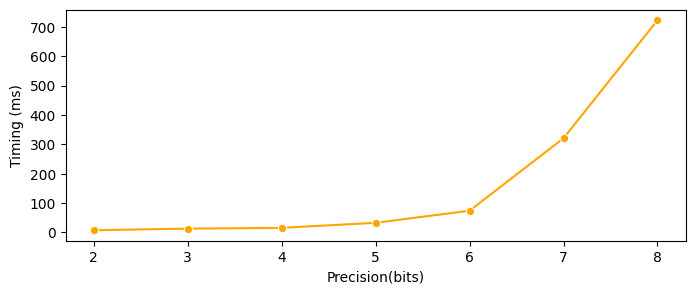
\includegraphics[width=0.8\linewidth]{tex/larger_luts/Figures/timings_pbs_precisions.png}
	\caption{Timings of the PBS with respect to $\log_2(p)$, where $p$ is the plaintext modulus}
	\label{fig:PBS_perfs}
\end{figure}



Intuitively, the reason is simple. When one wants to use a greater $p$, the torus must be sliced into more parts, that are thus smaller. When we switch the modulus to $2N$ in the bootstrapping, the ``windows'' of the accumulator polynomial gets smaller, so the bound on the noise to ensure correct bootstrapping must be smaller. To keep some room to enable the homomorphic capabilities of TFHE, one has to pick a greater value for the degree $N$. As this must be a power of two, it quickly reach values where the polynomial operations gets very slow.

Usually, PBS is not used for plaintext modulus greater than 8 bits. Some constructions exist in the literature to extend the capabilities of this algorithm to larger plaintext spaces, notably the tree bootstrapping of \cite{TCHES:GuiBorAra21} and the WoP-PBS of \cite{AC:CLOT21}. In this thesis, we propose our own in Chapter \ref{chap:larger_lut}.







%!TEX root = ../thesis.tex

\chapter[The Negacyclicity Problem]{Overcoming the Negacyclicity Problem with an Odd Plaintext Modulus}
\label{chap:negacyclicity}


In Section \ref{sec:pbs}, we presented the algorithm of the \gls{PBS}. But we left a question unanswered: what is the actual composition of the accumulator polynomial $\acc$? This is a tricky question, because this definition depends on the countermeasure picked against the negacyclicity problem (that we briefly introduced in Section \ref{sec:overview_blind_rotation}). 


In this chapter, we formalize the negacyclicity problem. We then present the classical countermeasure (the strategy of the padding bit), and our technique of odd plaintext modulus, which is a foundational block for the following contributions presented in this thesis. We finish by going through several others works that propose different countermeasures.


\section{Basics on Negacyclicity}

\paragraph{What is negacyclicity ?}

Let $v(X)$ be a polynomial of the ring $\glweRing$, such that $v(X) = \sum_{k=0}^{N-1} v_k X^k$. Recall how a multiplication by $X$  in this ring ``rotates'' the coefficients of the polynomial: \[X \cdot v(X) = - v_{N - 1} + v_0 \cdot X \dots + v_{N - 2} X^{N - 1}~.\]

In \gls{TFHE}'s blind rotation, the polynomial multiplication is done by the monomial $X^{-\Tilde{\mu}}$, with $\Tilde{\mu} \in \left \lbrace 0, \dots, 2N - 1 \right \rbrace$. This leads to two problems:

\begin{itemize}
	\item A coefficient $v_j$ can be brought in first place by two different rotations: the one induced by the polynomial multiplication by $X^{\modulo{-j}{2N}}$ and the one by $X^{[-j + N]_{2N}}$. It means that two different messages produce the same output.
	\item Each time a coefficient goes last to first, it gets negated (because $X^N = -1$ in the ring). So actually, the multiplication by $X^{[-j]_{2N}}$ yields correctly $v_j$, but the one by $X^{[-j + N]_{2N}}$ yields $-v_j$.
\end{itemize}


As the actual value of $\tilde{\mu}$ is encrypted, this is not possible to predict beforehand whether this undesirable minus sign will appear or not. So a countermeasure needs to be implemented into the scheme to neutralize the negacyclicity problem. The most frequent strategy is to develop encodings for the \gls{LUT} $f$ in the accumulator specifically tailored to handle this issue.


\paragraph{The ``natural'' case.}

Some functions interact naturally very well with the blind rotation algorithm: these are called the \textit{negacyclic functions} and they are presented in Definition \ref{def:negacyclic_function}.


\begin{definition} (Negacyclic Function)
	Let $p$ and $p'$ be two positive integers, with $p$ even. A function $f : \Z_p \mapsto \Z_{p'}$ is negacyclic if and only if it satisfies the following property:
	
	\[
		\forall x \in \Z_p, f\left (\modulo{x + \frac p 2}{p} \right ) = \modulo{-f(x)}{p'}
	\]
	
	\label{def:negacyclic_function}
\end{definition}


With such functions, the accumulator is quite simple to build: intuitively we only fill it with the values of the first half of the torus (so the $f(x)$ with $x \in \left [0, \frac p 2 - 1 \right ]$). So, if we rotate by the value corresponding to $i \ge \frac p 2$, a minus sign appears and we retrieve correctly $-f\left(i - \frac p 2 \right)$ .

We give an explicit formula for this accumulator in Definition \ref{def:negacyclic_accumulator}

\begin{definition} (Negacyclic Accumulator)
		\label{def:negacyclic_accumulator}
		Let $p$ and $p'$ be two positive integers, with $p$ \textbf{even}. Let $f:\Z_p \mapsto \Z_{p'}$ be a negacyclic function. Let $N$ be a power of two. Then, the accumulator $\acc$, defined by:
	
	\[
		\acc^{\textsf{negacyclic}} = X^{\frac{-2N}{2p}} \cdot \sum_{j=0}^{2N / p - 1} X^j \cdot \sum_{i=0}^{p/2 - 1} f(i) X^{i \frac{2N}{p}} \mod (X^N + 1)
	\]
	
\noindent is a valid accumulator for the blind rotation. It means that running the $\BlindRotate$ algorithm with this accumulator yields the right value.
	
	\paragraph{Remark on the encoding:}
	$f(i)$ is an element of the plaintext space $\Z_p$. In the context of this definition, we refer to its encoding into the ciphertext space $\Z_q$ (according to the procedure of Section \ref{sec:encryption}). That is to say, we actually put $\rounding{\frac{f(i) \cdot q}{p}}$ in the coefficients of the polynomial.
\end{definition}



Unfortunately, this construction is merely theoretical. Indeed, in practical setting, restricting the functions to be evaluated by \gls{PBS} only to negacyclic function greatly limits the capability of the scheme. In order to be able to evaluate \textit{any} function in the \gls{PBS}, more sophisticated techniques are required. We introduce the first example of such technique in the next section.


\section{The Classical Countermeasure: the Bit of Padding}
\label{sec:bit_of_padding}

The first countermeasure, that already appeared in the original \gls{TFHE} paper, is called the \textit{bit of padding}. As in the ideal case presented in the previous section, it works in an \textbf{even} plaintext space.

The idea is to ensure that the message stays in the first half of the torus all along the computations. An equivalent way of presenting it is to force the Most Significant Bit (\gls{MSB}) of the message to zero. By doing this, the modswitched phase used as the exponent in the blind rotation $\tilde{\mu}$ lives in $\{0, \dots, N - 1\}$, so the arising minus signs never reach the degree-zero coefficient.

The advantage of this method is that it relaxes the negacyclicity constraint and makes the bootstrapping able to evaluate any function (not only the negacyclic one). However, this construction is rather fragile: any linear function can break it by propagating a carry into the \gls{MSB}. 

To avoid this, when evaluating an homomorphic circuit, the program needs to keep track of the maximal value that each homomorphic operation can yield and make sure that it will never propagate a carry into the \gls{MSB}. This often leads to extra bootstrapping to control the growth of the message and eliminate the overflows. 


In the following, we give the definition of the accumulator $\acc$ in this ``bit-of-padding'' case:

\begin{definition}(Bit-of-Padding accumulator)
	Let $p$ and $p'$ be two positive integers, with $p$ \textbf{even}. Let $f: \Z_p \mapsto \Z_{p'}$ be a function. Let $N$ be a power of two. Then, the accumulator $acc(X)$:
	\[
		\acc^{\textsf{bit-of-padding}} = X^{\frac{-N}{2p}} \cdot \sum_{j=0}^{N / p - 1} X^j \cdot \sum_{i=0}^{p - 1} f(i) X^{i \frac{N}{p}} \mod (X^N + 1)
	\]
	
\noindent is a valid accumulator for the blind rotation.
	\paragraph{Remark on the encoding:}
	Contrary to the purely negacyclic case of Definition \ref{def:negacyclic_accumulator}, $f(i)$ is not encoded in the Most Significant Bits of the polynomial's coefficient. Instead, the \gls{MSB} is reserved and fixed to zero to maintain the encoded value in the first half of the torus. That is to say, we actually put $\rounding{\frac{f(i) \cdot q}{2 \cdot p}}$ in the coefficients of the polynomial.
\end{definition}


An example of such an accumulator is shown on Figure \ref{fig:negacyclic_accumulator}.

\begin{figure}[H]
	\centering
	\begin{tikzpicture}
		\drawHalfRing{4}{small}{true}{true}{true}
		\drawSingleRingHalfColor{64}{4}{big}{true}{false}{true}
	\end{tikzpicture}
				
	\vspace{1.5em}
	
	\textbf{Bit-of-Padding Accumulator:}\\[0.5em]
	\negacyclicAccumulator{4}{32}
	
	\caption{An example of bit-of-padding accumulator, with $p=4$ and $N = 32$. Hatching shows the parts which have an additional minus signs.}
	\label{fig:negacyclic_accumulator}
\end{figure}





The drawback of the bit-of-padding padding makes very challenging the development of homomorphic applications, because it prevents to use the linear operations freely. One should keep track of the maximal value contained in a ciphertext to avoid an overflow that would fill the padding bit. In Chapter \ref{chap:p_encodings}, we will demonstrate how this method makes the evaluation of Boolean circuit very inefficient, and we propose a new method that improves it.

Other constructions have been developed to avoid these drawbacks, we present them in Section \ref{sec:soa_padding_bit}.



\section{Other Countermeasures Avoiding the Bit of Padding}
\label{sec:soa_padding_bit}

Because the classical bit-of-padding solution brings too many constraints on the evaluation of computational circuits, several alternative constructions have been proposed to homomorphiclaly evaluate \gls{LUT}. To do so, many of these constructions adopt a similar strategy: they decompose the target function into a sequence of several \gls{PBS} steps. 

A notable line of work, including \cite{EPRINT:YXSCZ21}, \cite{AC:LiuMicPol22}, and \cite{TCHES:KluSch23}, employs a two-step \gls{PBS} strategy. In these approaches, the first \gls{PBS} evaluates a quantity  encrypting the bit indicating whether the message lies in the positive or negative half of the torus. This effectively extracts the ``sign'' of the message. The second \gls{PBS} then evaluates the actual function of interest regardless of the effects of negacyclicity, producing a result that may be flipped in sign. The ambiguity introduced by this flip is corrected using the result of the first \gls{PBS}. While the specific techniques used to perform this correction vary across works, the overall architecture remains the same: use the first \gls{PBS} to identify the torus half, and use this information to rectify the sign of the second \gls{PBS} output.

Another interesting approach is presented in \cite{AFRICACRYPT:CBSZ23}, where the target function is expressed as a sum of functions sharing a particular structure: so-called \textit{pseudo-odd} and a \textit{pseudo-even} function. These two properties are special cases of negacyclic functions, so they allow an evaluation with a \gls{PBS} without suffering from the negacyclicity issue. Although this decomposition may require more than two \gls{PBS} calls, an important advantage of the method is that the evaluations can be carried out in parallel. This contrasts with the previously mentioned approaches, which are intrinsically sequential due to the dependency between the two \gls{PBS} stages.

A completely different line of work is explored in \cite{AC:CLOT21}, which introduces the “Without-Padding \gls{PBS}” (WoP-\gls{PBS}) construction. A more refined version of this technique is presented in \cite{JC:BBBCLO23}, and we describe it here. The method begins by evaluating a scaled sign function (that is inherently negacyclic) using a standard \gls{PBS}. Following this, the individual bits of the message are extracted and converted into $\GGSW$ ciphertexts (see Definitions \ref{def:ggsw} and \ref{def:ggsw2}) using a procedure known as \textit{circuit bootstrapping}. These ciphertexts are then used as selectors in a graph of $\CMUX$ operations (Definition \ref{def:cmux}) to select an appropriate accumulator based on the high-order bits of the message. Finally, a traditional \gls{PBS} is used to rotate the selected accumulator according to the remaining lower-order bits.

Although this technique is slower for small plaintext sizes, it scales particularly well with an increasing plaintext sizes. Notably, it enables the homomorphic evaluation of LUTs with larger plaintext sizes beyond what is feasible with classical \gls{PBS} techniques, up to approximately 20 input bits.


In this thesis, we focus on a method we introduced in \cite{TCHES:BonPoiRiv24}: \textit{the odd plaintext modulus}.

\section{Our Contribution: the Odd Plaintext Modulus}
\label{sec:odd_modulus}

Negacyclicity has a quite different effect depending of the parity of the plaintext modulus $p$. Recall that $\mu = m + e \in \Z_q$, with $e$ sampled from a small centered Gaussian. Because the error is small, $\mu$ does not take all the values of $\Z_q$ with the same probability: in particular, the densest parts in terms of probability over $\Z_q$ are the one close to the ``noiseless'' encodings of $m$, namely $\left \{ \rounding{\frac {k q}{p}} ~\middle |~ k \in \Z_p \right \}$. We illustrate this distribution on Figure \ref{fig:density_of_phase}. We call these sections of the torus the \emph{dense spots}.


\begin{figure}[h]
	\centering
	\begin{minipage}{0.47\textwidth}
		\centering
		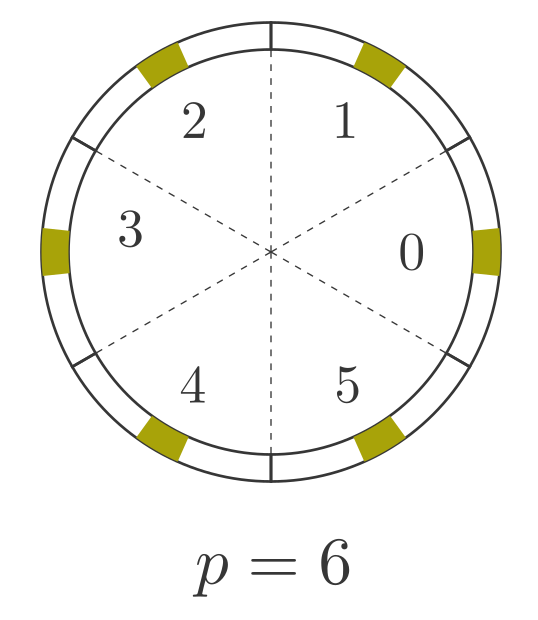
\includegraphics[width=0.8\textwidth]{img/to_harmonize/busy_sectors_2.png}
	\end{minipage}
	\hspace{0.04\textwidth}
	\begin{minipage}{0.47\textwidth}
		\centering
		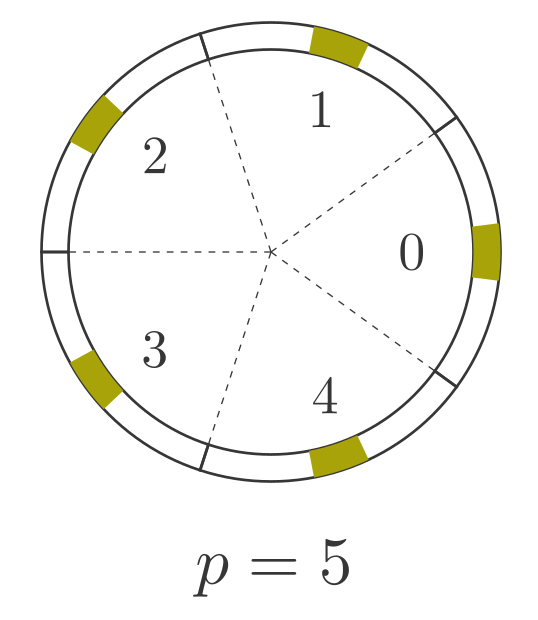
\includegraphics[width=0.8\textwidth]{img/to_harmonize/busy_sectors.png}
	\end{minipage}
	\caption{Distribution of the values of $\mu$ across $\mathbb{Z}_q$ for $p = 6$ and $p = 5$: the colored parts show the dense spots where the value has a high probability to lie in. The width of these sectors depends on $\sigma$ (the standard deviation of the error distribution $\chi$ of \gls{TFHE}). Note that this repartition looks similar for $\Tilde{\mu}$ in $\mathbb{Z}_{2N}$.}
	\label{fig:density_of_phase}
\end{figure}


When we transpose these dense spots into $\Z_{2N}$, they become the sectors close to $\left \{ \rounding{\frac{k \cdot 2N}{p}} \mid k \in \Z_p \right \}$. 

Let $k \in \Z_p$, the multiplication $X^{- \frac{k \cdot 2N}{p}} \cdot v(X)$ in the ring $\glweRing$ yields the same degree-zero coefficient as the multiplication  $X^{\modulo{- \frac{k \cdot 2N}{p} + N}{2N}} \cdot v(X)$, up to the minus sign. To make the rest of this section clearer, we change a bit the writing of the exponent as such: 
\[\modulo{
	\frac{
		-k \cdot 2N
	}
	{
		p
	}
	+ N
}{2N} = 
\modulo{
	\frac{
		(-k + \frac p 2 ) \cdot 2N
	}
	{p}
}
{2N}\]


This is where the parity of $p$ plays a part: if $p$ is even, then $\modulo{
	\frac{
		(-k + \frac p 2 ) \cdot 2N
	}
	{p}
}
{2N}$ is a dense spot as well. So collisions happen with high probability.  On the other hand, let us consider an odd value for $p$. Then, $\modulo{
	\frac{
		(-k + \frac p 2 ) \cdot 2N
	}
	{p}
}{2N}$ is no longer a dense spot, as it lies exactly halfway between the two dense spots $\modulo{
	\frac{
		(-k + \frac {p-1} {2} ) \cdot 2N
	}
	{p}
}{2N}$ and $\modulo{
	\frac{
		(-k + \frac {p+1} {2} ) \cdot 2N
	}
	{p}
}{2N}$. As a consequence, collisions never occur. Figure \ref{fig:torus_p_even_vs_odd} illustrates this phenomenon.


\begin{figure}
	\begin{subfigure}{0.49\linewidth}
		    \centering
		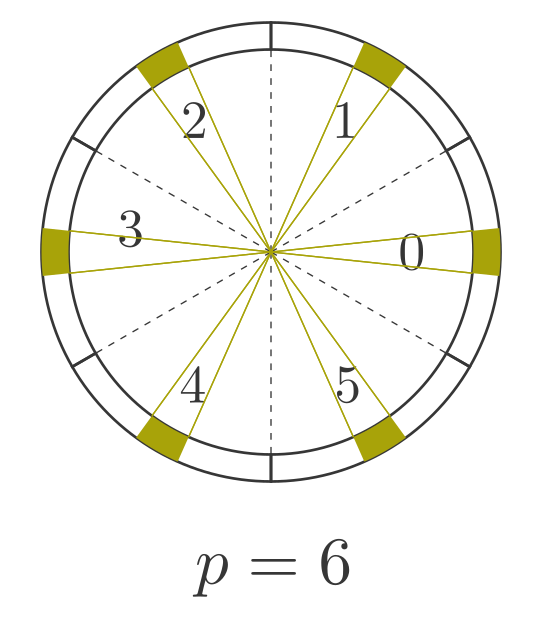
\includegraphics[width=0.5\linewidth]{img/to_harmonize/torus_p_even.png}
		\caption{With $p$ even, the dense spots of each half of the torus are aligned.}
		\label{fig:torus_p_even}
	\end{subfigure}\hspace{1em}% Adjust the margin width as needed
	\begin{subfigure}{0.49\linewidth}
		\centering
		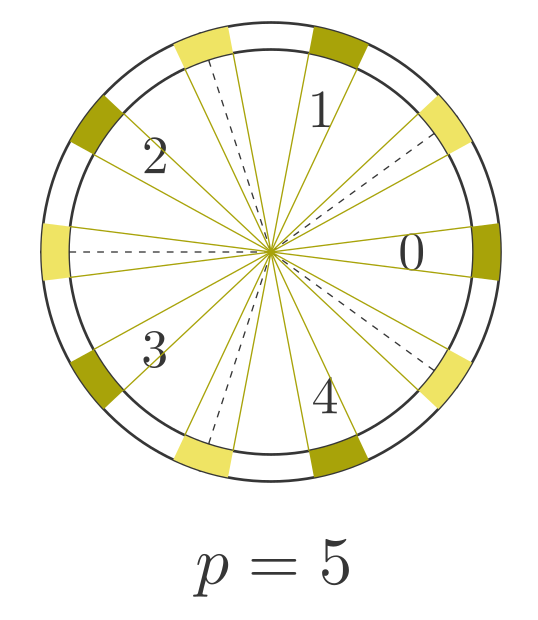
\includegraphics[width=0.5\linewidth]{img/to_harmonize/torus_p_odd.png}
		\caption{With $p$ odd, the dense spots face empty spots, close to the bounds of the $p$-sectors.}
	\end{subfigure}
	\caption{}
	\label{fig:torus_p_even_vs_odd}
\end{figure}



So, by selecting odd values for the plaintext modulus, the negacyclicity problem is naturally neutralized.


We present in Definition \ref{def:odd_accumulator} the formula for the accumulator in this case. Note that because $N$ is a power of two and $p$ an odd value, some rounding is required in the quotient $\frac N p$, but we omit it to keep notations lighter, (or equivalently, the division operator is assumed to include rounding).

\begin{definition}(Odd-case Accumulator)
	\label{def:odd_accumulator}
	Let $p$ and $p'$ be two integers, with $p$ \textbf{odd}. Let $f: \Z_p \mapsto \Z_{p'}$ a function, and $N$ a power of two. Then, the accumulator $\acc \in \glweRing$ has the form:
	\[
		\acc^{\textsf{odd-modulus}} = X^{- \frac {N} {2p}} \cdot \sum_{j=0}^{N/p - 1} X^j  \cdot \left ( \sum_{i=0}^{\frac{p-1}{2}} f(i) X^{i \frac{2N}{p}} + \sum_{i=0}^{\frac{p-1}{2} - 1} -f \left (i + \frac{p+1}{2} \right ) X^{i \frac{2N}{p} + \frac N p} \right )
	\]
	
	\paragraph{Remark on the encoding:}
	With this construction, we do not need a bit of padding anymore. So, the values $f(i)$ are encoded using the simple encoding of Section \ref{sec:encryption}, that is to say $\rounding{\frac{f(i) \cdot q}{p}}$.
\end{definition}



Let us explain the structure of this accumulator. The polynomial has degree $N$ and is made of $p$ distinct windows of width $\frac{N}{p}$. Each of these windows has constant coefficient value $f(k)$, for $k \in \{0, \dots, p-1\}$.
For $0 \le \alpha \le \frac{p-1}{2}$, the range of degrees whose coefficients are $f(\alpha)$ is $\left [ \alpha \frac{2N}{p} - \frac{N}{2p}~;~ \alpha \frac{2N}{p} + \frac{N}{2p} \right ]$. Now, for $\frac{p+1}{2} \le \beta \le p-1$, we can write $\beta = \alpha + \frac{p+1}{2}$, with $0 \le \alpha < \frac{p-1}{2}$. This time, the range of spanned degrees is $\left [ \alpha \frac{2N}{p} + \frac{N}{2p} ~;~ (\alpha + 1) \frac{2N}{p} - \frac{N}{2p} \right ]$. Thus, the values $k \in \{0, \dots, p-1\}$ spans the entire space $[0; N)$ without overlap. The values over $\frac{p+1}{2}$ gets negated by the negacyclicity, so the underlying coefficient is also negated to compensate this effect. We illustrate this construction on Figure \ref{fig:accumulator_odd}.




\begin{figure}[H]
	\centering
	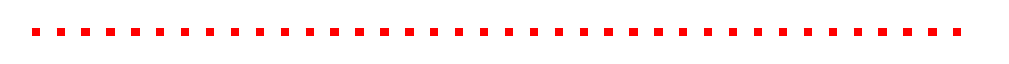
\begin{tikzpicture}
		\drawSingleRing{5}{5}{small}{true}{true}{true}
		\drawRingOddEncoding{64}{5}{big}{true}{false}
		\draw[red, loosely dashed, line width=1mm] (-6,0) -- (6,0);
	\end{tikzpicture}
	
	\vspace{1.5em}
%	
	\textbf{Odd-Modulus Accumulator:}\\[0.5em]
	\oddAccumulator{5}{32}
%	
%	\vspace{1.5em}
%	\textbf{Rotated by $N$:}\\
%	\oddAccumulatorInverted{5}{32}
	\caption{Illustration of the construction of the Odd-Modulus accumulator. On top is the ring $\Z_{2N}$ splitted in windows. Below is a representation of the polynomial $v$, with its version once rotated by a multiplication by $X^N$. On the figure, $p = 5$ and $N = 32$. Hatching shows the parts which have an additional minus signs}
	\label{fig:accumulator_odd}
\end{figure}


If we compare this approach to the bit-of-padding one, the windows have half the size. So we may think that the bound on the maximal noise to ensure correctness must be twice tighter. However, because the bit-of-padding accumulator makes use of only one half of the torus, the windows actually have the same width if we consider the same size of plaintext space. In Section \ref{sec:parametrization}, we elaborate further on how the parametrization of the scheme is handled in this case.


With this technique, no bit of padding is required. Consequently, it allows to use the linear homomorphisms without worrying about carry propagation. This is a key improvement that is at the root of the works presented in the rest of this thesis.





\section{Conclusion}

Our idea of employing odd plaintext moduli that we developed in Section \ref{sec:odd_modulus} do not have any computational overhead with respect to the classical bit-of-padding technique of Section \ref{sec:bit_of_padding}, while removing all the constraints the latter put on the homomorphic compilation. This is not the case of the other methods of the state of the art that we summed up in Section \ref{sec:soa_padding_bit}, which all increase the amount of computation 

However, working with an odd modulus may seem unhandy: data types in programming are usually defined on a power-of-two modulus for example. But we show in the following chapters (Chapter \ref{chap:p_encodings}, \ref{chap:hyppogriph}, \ref{chap:transistor} and \ref{chap:larger_lut}) that this introduces new applications and homomorphic capabilities to \gls{TFHE}.



\chapter{A first application: Accelerating Boolean circuits evaluation with $p$-encodings}


\chapter{Accelerating AES evaluation}


\chapter{More efficient transciphering with Transistor}



\chapter{Accelerating large look-up tables}


\chapter{Practical solution to the problem of parameter selection}
%...
%\chapter*{Conclusion}
\addstarredchapter{Conclusion}

Fully Homomorphic Encryption is believed to be on the verge of practical usability. But still some challenges are remaining so it can be used in our day-to-day life. In the following, we show how the works presented in this thesis adresses in these issues.

The purpose of this thesis was to adress some concrete obstacles that hinder the practical deployment of \gls{FHE}. In this concluding section, we list the main challenges and relate them to the contributions presented throughout this manuscript.

\paragraph{On Efficiency.}

\gls{FHE} still incurs an significant computational overhead compared to traditional, unencrypted computation. While the \gls{FHE} schemes themselves have been seen much improvement in the last years, an orthogonal direction is to design new algorithms tailored for specific use-cases. In Chapter \ref{chap:p_encodings}, we developed a framework to accelerate the evaluation of Boolean functions. At the opposite end of the spectrum, Chapter \ref{chap:larger_lut} focus on accelerating the evaluation of \gls{LUT} in larger plaintext spaces than those originally supported by \gls{TFHE}. Chapter \ref{chap:hyppogriph} further demonstrated how Boolean and arithmetic representations offer complementary advantages, and how efficient conversion mechanisms between both can enhance performance within homomorphic circuits. 

Another way of improving performances lies in selecting appropriate parameters for the scheme. We propose such a procedure of parameter selection, which takes into account the computational circuit to evaluate as well as the environment of execution.


\paragraph{On Data Expansion and Transciphering.}


Data expansion is another well-known bottleneck in \gls{FHE}. The literature has long proposed transciphering as a promising solution, however this technique necessitates homomorphic evaluation of the decryption function of a symmetric cipher. In Chapter \ref{chap:hyppogriph}, we have shown how far we could push to evaluate efficiently the \gls{AES} cipher using \gls{TFHE}. However, it is clear that standard ciphers such as \gls{AES} cannot compete against schemes specifically designed with the use-case of transciphering in mind. In Chapter \ref{chap:transistor}, we present such a cipher and show how its design combines the properties required to ensure both cryptographic security and homomorphic efficiency. 




\paragraph{On Compilation and Development of Homomorphic Computations.}
%

Developing homomorphic applications remains a tedious task, requiring deep understanding of both cryptography and the internal workings of specific \gls{FHE} schemes. It is clear that an adoption of \gls{FHE} at scale will require an automated compilation toolchain that will abstract away cryptography complexities from non-expert programmers.

In Chapter \ref{chap:p_encodings}, we proposed algorithm that automatically compiles Boolean functions into optimized sequences of homomorphic operations. We did a similar thing in the case of large LUTs in Chapter \ref{chap:larger_lut}, where those LUTs are compiled into a more tractable algorithm, composed of smaller ones. Finally, our parameter selection framework presented in \ref{chap:parameters} further contributes to this effort.


\bigskip

The road is probably still long until \gls{FHE} becomes an ubiquitous technology. But the pace of scientific progress in this field is accelerating rapidly. So it is reasonable to believe (and hope) that such a technological revolution will happen in a not-so-distant future.






%\appendix
%% !TeX root = ./main.tex
%% \section{Statistical independance of secret key and output key stream}
%% \ac{Je pense qu'il faut enlever cette section}
%% The independence between the key and the output key stream can be expressed by the following theorem.

%% \begin{lemma}
%% Let $n \in \mathbb{N}$ and let $F^{(n)}$ be the augmented function as defined in Section~\ref{sec:security-linear}. Let $X$ be the uniform random variable in $\mathbb{F}_p^{16}$ and let $S$ be the random variable in $\mathbb{F}_p^{4n}$ corresponding to the output of $F^{(n)}$ and let $K$ be the random variable corresponding to the secret key. If $F^{(n)}$ is balanced for all key, then
%% $$H(\keyvar |\outvar) = H(\keyvar )\,,$$
%% where $H$ is the entropy.
%% \end{lemma}

%% \begin{proof}
%% First, it is known that if the events $\keyvar = \keyevent$ and $\outvar = \outevent$ for all $\keyevent \in \mathbb{F}_p^{16(n-1)}$ and for all $\outevent \in \mathbb{F}_p^{4n}$ are independent then the result holds. 

%% Let $K^0 \in \mathbb{F}_p^{n-1}$ and $S^0 \in \mathbb{F}_p^{4n}$. We have 
%% $$\mathrm{Pr}[S= S^0 | K = K^0] = \mathrm{Pr}[S^0 = F^{(n)}(X,K_0^0,\ldots,K_{n-1}^0)] = \frac{1}{p^{4n}}\,.$$
%% The last equality comes from the hypothesis that $F^{(n)}$ is balanced for all possible keys. We eventually obtain independence between the output and the key.
%% \end{proof}

%%%
\section{Complexity of Correlation Attacks over \(\F_p\)}
\label{sec:complexity-correlation}

%\ac{Ce qui suit est encore en vrac}

\subsection{Proof of Proposition~\ref{prop: approx}}
\begin{figure}[b!]
\newcommand{\blue}[1]{\color{blue}#1}
\newcommand{\red}[1]{\color{red}#1}
    \centering
    \begin{tikzpicture}[xscale=.9]
      \footnotesize
      % variables
      %\draw ( 2, 0) node(Xt){$X_{t}$} ;
      \draw (-1.7, 0) node(U){$U$} ;
      \draw (11.5, 0) node(Xtplus){$X$} ;
      \draw (8, 1.5) node(Kt){$K$} ;
      % \draw (4.5, 1.5) node(St){$S_t$};
      % operations
    \draw (-1, 1) rectangle +(1, 1) node[pos=0.5]{$G_{1}$} ;
  \draw ( 0, -0.5) rectangle +(1, 1) node[pos=0.5]{$G_{2}$};
      \draw (3.5, 1) rectangle +(1, 1) node[pos=0.5]{$\filter$} ;
      \draw ( 6, -0.5) rectangle (7, 0.5) node[pos=0.5]{$L$} ;
      \draw (8, 0) node(add)[inner sep=0pt]{$\boxplus$} ;
      \draw (9, -0.5) rectangle (10, 0.5) node[pos=0.5]{$\subW$} ;
      % arrows
      \draw[->] (-.5, 0) -- (-.5, 1) ;
      \draw[->] (-1.5, 0) --  node[below,pos=.3] { $\blue{a}$} (0, 0) ;
      \draw[->] (1, 0) --  node[below, pos=.31] { $\red{L^{\top}(\alpha) + \filter^{*}(\beta')}$} node[below, pos=.85] { $\red{L^{\top}(\alpha)}$} (6, 0) ;
      \draw[->] (4, 0) -- node[left,pos=.7] {$\red{\filter^{*}(\beta')}$} (4, 1) ;
      \draw[->] (7, 0) --  node[below] {$\red{\alpha}$} (add) ;
      \draw[->] (Kt) -- node[left,pos=.2] {$\blue{\alpha}$}(add) ;
      \draw[->] (add) -- node[below] {$\red{\alpha}$} (9, 0) ;
      \draw[->] (10, 0) --  node[below] {$\blue{b}$} (Xtplus) ;
      \draw[->] (4, 2) -- node[left,pos=.5] {\blue{$\beta'$}} (4, 2.5) node[above] {};
    \draw[->] (-.5, 2) -- node[left,pos=.5] {\blue{$\beta$}} (-.5, 2.5) node[above] {};
    \draw[dashed] (1.2,-.5) -- +(0, 3);
    % masks
    \end{tikzpicture}

  \caption{Masks propagation through a composition with \coolName{}'s round function. Input and output masks are written in blue while inner masks whose value are deduced are written in red.\label{fig:masks}}
\end{figure}
\begin{proof}
  For \(n\)~rounds, the Fourier coefficient $\widehat{F_{\alpha, \beta}}(0,\lambda)$ corresponds to a Fourier coefficient of the following function
    \[\begin{array}{rccl}
H^{(n)}: & \F_p^{16} \times \F_{p}^{16(n-1)} & \rightarrow & \F_{p}^{4(n-1)} \times \F_p^{16}\\
& (X_{0}, K_{1}, \ldots, K_{n-1}) & \mapsto & (S_0, \ldots, S_{n-2},X_{n-1})\;.
     \end{array}\]
 In other words, the output of \(H^{(n)}\) corresponds (up to a reordering of the 16 last digits) to the concatenation of the output of the augmented function \(F^{(n)}\) and of the remaining 12~internal digits that are not output by~$\filter$. % the last state of the FSM which are not outputted by~\(\filter\).
 Then, \(H^{(n+1)}\) can be seen as the composition of \(H^{(n)}\) with the round function
 \[\begin{array}{rcl}
 \F_p^{16} \times \F_p^{16} & \rightarrow & \F_p^4 \times \F_p^{16}\\
 (X_{n-1},K_n) & \mapsto & \left(\filter(X_{n-1}), \subW(L(X_{n-1})+K_n)\right)\end{array}\]
 Let \(G\) be any function of the form
 \[\begin{array}{rcl}
 G:\F_p^{\ell} & \rightarrow & \F_p^k \times \F_p^{16}\\
 U & \mapsto & (G_1(U),G_2(U))\end{array}\;.\]
 Then, the Fourier transform of the composition
 \[F:(U,K) \mapsto (G_1(U), \filter(G_2(U)), \subW(L(G_2(U))+K))\]
 can be easily derived from the Fourier transform of~\(G\), as shown on Figure~\ref{fig:masks}.
 Indeed, the detailed computation of the Fourier coefficient
 \[\mathcal{I} := {\widehat F}(a, \alpha;\beta, \beta', b)\]
 for the input mask \((a, \alpha)\) and output mask \((\beta, \beta', b)\) is as follows.
 \begin{eqnarray*}
   \mathcal{I} & = & \sum_{U \in \F_p^\ell,K \in \F_p^{16}} \omega^{\beta \cdot G_1(U) + \beta' \cdot \filter(G_2(U)) + b \cdot \subW(L(G_2(U))+K) - \alpha \cdot K - a \cdot U} \\
   & = & \sum_{U \in \F_p^\ell} \omega^{\beta \cdot G_1(U) + \beta' \cdot \filter(G_2(U))- a \cdot U} \left(\sum_{Z \in \F_p^{16}} \omega^{b \cdot \subW(Z) -\alpha \cdot Z+ \alpha \cdot L(G_2(U))}\right)
 \end{eqnarray*}
 where we set \(Z = L(G_2(U))+K\).
 We then deduce
 \begin{eqnarray*}
   \mathcal{I} & = & \sum_{U \in \F_p^\ell} \omega^{\beta \cdot G_1(U) + \beta' \cdot \filter(G_2(U))- a \cdot U + \alpha \cdot L(G_2(U))} {\widehat \subW}(\alpha, b)\\
   & = & {\widehat \subW}(\alpha, b)\sum_{U \in \F_p^\ell} \omega^{\beta \cdot G_1(U) + \filter^*(\beta') \cdot G_2(U)- a \cdot U + L^T(\alpha) \cdot G_2(U)} \\
   & = & {\widehat \subW}(\alpha, b) {\widehat G}(a ; \beta, L^T(\alpha) + \filter^*(\beta'))
   \end{eqnarray*}
 where \(\filter^*: \F_p^4 \rightarrow \F_p^{16}\) is the function outputting an internal state whose digits are all zero, expect the digits affected by \(\filter\), which are equal to the inputs.
       Finally, we observe that \(H^{(1)}\) is the identity function implying that \({\widehat H^{(1)}}(a,b) = p^{16}\) if \(a=b\) and \(0\) otherwise.
       It follows that the Fourier coefficients of \(H^{(n)}\) are either zero, or given by % \jb{Il manque pas un $\ind{a}(b'_{0})$ du coup comme premier terme ?}
       \[{\widehat H^{(n)}}(a, \alpha_1, \ldots \alpha_{n-1}; \beta_0, \ldots, \beta_{n-2}, b) = p^{16} \prod_{i=1}^{n-1} {\widehat \subW}(\alpha_{i}, b'_i) \;,\]
       for some \(b'_1, \ldots, b'_{n-1}\).
       Therefore,
       \[p^{-16n} {\widehat H^{(n)}}(a, \alpha_1, \ldots, \alpha_{n-1}; \beta_0, \ldots, \beta_{n-2}, b) = \prod_{i=1}^{n-1} \frac{{\widehat \subW}(\alpha_{i}, b'_i)}{p^{16}} \;.\]
 %Note that $\widehat{F_{\alpha, \beta}}(0,\lambda)$ corresponds to a particular case of $\widehat H^{(n)}$.
   The result then directly follows by observing that \({\widehat \subW}(\alpha_{i}, b'_i)\) is the product of the Fourier coefficients of the 16~\gls{S-box}es composing \(\subW\).
\hfil\qed
  \end{proof}

%% Let $(a, \alpha_1, ..., \alpha_{n}; \beta_0, ..., \beta_{n-1})$ be a vector of masks where the semi-colon separates input ones from output ones. Let us begin by proving that there exists \(b' \in \F_p^{16}\) such that
%%      % \noindent
%%      % \scalebox{0.86}{
%%      {\footnotesize
%%      \begin{equation*}
%%          {\widehat H^{(n+1)}}(a, \alpha_1, ..., \alpha_{n}; \beta_0, ..., \beta_{n-1}, b) ~=~
%%          {\widehat H^{(n)}}(a, \alpha_1, ..., \alpha_{n-1}; \beta_0, ..., \beta_{n-2}, b') \times {\widehat \subW}(\alpha_{n}, b) .
%%        \end{equation*}
%%      }

   
%%      Let \(\omega\) be a \(p\)-th root of unity in~\(\mathbb{C}\) and \(\chi(x) = \omega^x\) for \(x \in \F_p\). Then,
     
%%        \begin{eqnarray*}
%%          \mathcal{I} & = &   {\widehat H^{(n)}}(a,\alpha_1, \ldots, \alpha_{n-1}; \beta_0, \ldots, \beta_{n-2},b') \times {\widehat \subW}(\alpha_{n}, b) \\
%%                      & = & \sum_{X_0, K_1, \ldots, K_{n-1}} \chi\left(\sum_{i=0}^{n-2}\beta_i \cdot S_i + b'\cdot X_{n-1}- \sum_{i=1}^{n-1} \alpha_i \cdot K_i- a \cdot X_0\right) \sum_{Z} \chi\left(b \cdot \subW(Z) - \alpha_n \cdot Z\right) \\
%%                      & = & \sum_{X_0 ,K_1, \ldots, K_{n-1},K_n }   \chi\left(\sum_{i=0}^{n-2}\beta_i \cdot S_i + b' \cdot X_{n-1} - \sum_{i=1}^{n-1} \alpha_i \cdot K_i - a \cdot X_0\right)\\
%%        & & \hspace*{2cm} \times \chi\left(b \cdot \subW(K_n+L(X_{n-1})) - \alpha_n \cdot K_n - \alpha_n \cdot L(X_{n-1})\right)\;,
%%        \end{eqnarray*}
%%        where the variables summed over go through $\F_p^{16}$, and the last equality is obtained by setting \(Z = K_n + L(X_{n-1})\). Let \(\filter^*: \F_p^4 \rightarrow \F_p^{16}\) be the function outputting an internal state whose digits are all zero, expect the digits affected by \(\filter\), which are equal to the inputs. By exchanging the positions of $ b' \cdot X_{n-1}$ and $b \cdot X_{n} = b \cdot \subW(K_n+L(X_{n-1}))$, adding $\alpha_n \cdot K_n$ to the sum of $ \alpha_i \cdot K_i$, and adding $\beta_{n-1}\cdot S_{n-1} = \filter^*(\beta_{n-1}) \cdot X_{n-1}$ to the sum of $\beta_{i}\cdot S_{i}$, we deduce that \ac{Je trouve ca mega complique. Pourquoi pas simplement: We can rewrite \(\mathcal{I}\) as follows.}
%%       \begin{eqnarray*}
%%        \mathcal{I} 
%%        & = & \sum_{X_0, K_1, \ldots, K_{n} \in \F_p^{16}}  \chi\left(\sum_{i=0}^{n-1}\beta_i \cdot S_i + b \cdot X_n - \sum_{i=1}^{n} \alpha_i \cdot K_i - a \cdot X_0\right) \\
%%             & & \quad \times \chi\left(b' \cdot X_{n-1} -\filter^*(\beta_{n-1})\cdot X_{n-1}  - \alpha_n \cdot L(X_{n-1})\right).
%%            \end{eqnarray*}
%%            \begin{eqnarray*}
%%          & = & \sum_{X_0, K_1, \ldots, K_{n} \in \F_p^{16}}  \chi\left(\sum_{i=0}^{n-1}\beta_i \cdot S_i  + b \cdot X_n - \sum_{i=1}^{n} \alpha_i \cdot K_i - a \cdot X_0\right)\\
%%        & & \quad\times \chi\left((b'-\filter^*(\beta_{n-1}) - L^T(\alpha_n)) \cdot X_{n-1}\right) \\
%%      & = &    {\widehat H^{(n+1)}}(a,\alpha_1, \ldots, \alpha_n; \beta_0, \ldots, \beta_{n-1},b) \;,
%%          \end{eqnarray*}
%%        when \(b'=\filter^*(\beta_{n-1}) + L^T(\alpha_n)\) and \(L^T\) is the transpose of~\(L\). 


   


\subsection{Data Complexity of Fast Correlation Attacks}
\label{sec:fast-correlation-data}

It is well-known that the capacity of a linear approximation determines the minimal length of the sequence obtained by a given linear combination of the digits of \((S_t)_{t \in \mathbb{N}}\) that is required for recovering the initial state of the key-LFSR from the linear approximation
\[\sum_{i=1}^{n-1} \alpha_i \cdot K_{t+i} + \sum_{i=0}^{n-1} \beta_i \cdot S_{t+i}, \forall t \geq 0\;.\]

However, the same result holds even when the approximation is not linear as stated in the following theorem.
\begin{theorem}\label{th:Nmin}
  Let  \(F\) be a function from \(\F_p^\kappa \times \F_p^m\) to \(\F_p^n\). Let \(g:\F_p^\kappa \rightarrow \F_p\) and \(h: \F_p^n \rightarrow \F_p\) such that the probability distribution of
  \[(U,V) \mapsto h(F(U,V)) - g(U)\]
  is close to the uniform distribution, \ie, for all \(z \in \F_p\),
  \[\pr_{(U,V) \drawfrom \F_p^\kappa \times \F_p^m}[h(F(U,V)) - g(U)=z] = \frac{1}{p} + \varepsilon_z \mbox{ with } \varepsilon_z\ll 1\;.\]
  Let \((U_t)_{t \in \mathbb{N}}\) be a sequence of elements in~\(\F_p^\kappa\) defined by \(U_{t+1} = \Phi(U_t)\), where  $\Phi$ is a function from $\F_p^\kappa$ to itself. Let \((V_t)_{t \in \mathbb{N}}\) be a sequence of elements in~\(\F_p^m\).
  Then, the minimal length \(N\) of the sequence \( (B_{t})_{t \in \mathbb{N}} \vcentcolon= \left( h(F(U_t,V_t) \right)_{t \in \mathbb{N}}\) 
    required for recovering \(U_0\) is
  \[N = \frac{\kappa \ln p}{\Delta}\]
  with \[\Delta = p \sum_{y \in \F_p} \varepsilon_y^2 = \sum_{a \in \F_p^*} \left|p^{-\kappa} \sum_{U \in \F_p^\kappa,V\in \F_p^m}\omega^{a(h(F(U,V)) - g(U))}\right|^2\;.\]
\end{theorem}
\begin{proof}
  Let
  \[\mathcal{C} = \{(g(\Phi^t(U_0)))_{0 \leq t < N}, U_0 \in \F_p^\kappa\}\;.\]
  This set is a (non-linear) code over \(\F_p\) of length~\(N\) and size \(p^\kappa\).
  As originally observed by Meier and Staffelbach~\cite{EC:MeiSta88}, recovering \(U_0\) from \((B_0, \ldots, B_{N-1})\) boils down to decoding this code. Indeed, \((B_0, \ldots, B_{N-1})\) can be seen as the result of the transmission of the \(N\)-digit word \((g(U_0), \ldots, g(\Phi^{N-1}(U_0)))\)  through a noisy transmission channel. This transmission channel is memoryless, since each digit is affected in the same way:
  \[B_t = g(\Phi^{t}(X_0)) + \eta_t\]
  where the probability distribution of all \(\eta_t\) is given by
  \[\pi_z := \pr[\eta_t = z] = \pr_{(U,V) \drawfrom \F_p^\kappa \times \F_p^m}[h(F(U,V)) - g(U)=z]= \frac{1}{p} + \varepsilon_z\;.\]
  This transmission channel is called symmetric in the sense that its transition matrix, formed by the probabilities that an input value~\(i\) is transformed to~\(j\), is a circulant matrix whose rows correspond to the probability distribution \((\pi_0, \ldots, \pi_{p-1})\).
  Therefore, Shannon's channel-coding theorem~\cite[Section~7.7]{add:CovTho06} implies that this code can be decoded with a non-negligeable success probability if and only if its rate, \ie, the ratio between the logarithm of its size and its length, is smaller than the channel capacity:
  \[\frac{\kappa}{N} \leq C_{\mathrm{channel}}\;.\]
  The capacity of any \(p\)-ary symmetric channel is given by~\cite[Th.~7.2.1]{add:CovTho06}
  \[C_{\mathrm{channel}} = 1 - H_p(\pi_0, \pi_1, \ldots, \pi_{p-1})\]
  where \(H_p\) denotes the \(p\)-ary entropy, i.e.,
  \[H_p(\pi_0, \pi_1, \ldots, \pi_{p-1}) := - \sum_{z \in \F_p} \pi_z \log_p(\pi_z)\;.\]
  We use that, for \(\varepsilon \ll 1\),
  \[\ln\left(\varepsilon + \frac{1}{p}\right) = \ln(1 + p \varepsilon) - \ln p = p \varepsilon - \ln p + o(\varepsilon)\;.\]
  It follows that
  \begin{eqnarray*}
    \sum_{z \in \F_p} \left(\varepsilon_z + \frac{1}{p}\right) \ln\left(\varepsilon_z + \frac{1}{p}\right) & \simeq & p \sum_{z \in \F_p} \varepsilon_z^2 - \ln p \sum_{z \in \F_p} \left(\varepsilon_z + \frac{1}{p}\right)\;.
  \end{eqnarray*}
  We then deduce that
  \[C_{\mathrm{channel}} = 1 + \frac{1}{\ln p} \left(p \sum_{z \in \F_p} \varepsilon_z^2  -\ln p\right) = \frac{1}{\ln p} \left(p \sum_{z \in \F_p} \varepsilon_z^2\right)\;.\]
  It is well-known (see Prop.~\ref{prop:capa}) that the same quantity can also be derived from the Fourier transform of the function
  \[f: (U,V) \mapsto h(F(U,V)) - g(U)\;.\]
  Indeed, if \(\pi'\) denotes the function from \(\F_p\) to \(\mathbb{R}\) defined by \(\pi'(x) = \pi_x - \frac{1}{p} = \varepsilon_x\), we have
    \[\Delta = p \sum_{y \in \F_p} \left|\pi'(y)\right|^2 = \sum_{a \in \F_p} \left|{\widehat \pi'}(a)\right|^2\]
    where the last equality corresponds to Plancherel's formula.
    Moreover, the Fourier transform of~\(\pi'\) an be computed as follows: if \(a \neq 0\),
    \begin{eqnarray*}
      {\widehat \pi'}(a) & = & \sum_{x \in \F_p} \pi'(x) \omega^{-ax} = \sum_{x \in \F_p} \pi_x \omega^{-ax} - p^{-1} \sum_{x \in \F_p} \omega^{-ax}\\
      & = & p^{-(\kappa+m)} \sum_{x \in \F_p} \#f^{-1}(x) \omega^{-ax} = p^{-(\kappa+m)} \sum_{U,V \in \F_p^\kappa \times \F_p^m}  \omega^{-a f(U,V)}
      \\ & = & p^{-(\kappa+m)} {\widehat f}(0, -a)\;,
      \end{eqnarray*}
    and \({\widehat \pi'}(0) = 0\).
        It follows that
        \[\Delta = \sum_{a \in \F_p^*} \left|p^{-(\kappa+m)} {\widehat f}(0, a)\right|^2\;.\]
        \hfil\qed
\end{proof}



% Leo: ce qui suit est pour qu'emacs compile bien l'article, pas touche !
%%% Local Variables:
%%% mode: latex
%%% ispell-local-dictionary: "english"
%%% TeX-master: "main"
%%% End:


% =============================================
%                 END
% =============================================

\bibliographystyle{alpha}
\bibliography{cryptobib/abbrev0, cryptobib/crypto, add}

%==============================
\end{document}